% 2023本郷祭 マイコン部 部誌 「マイコンHONGOMagazine」 TeXテンプレート

% =環境設定=

\documentclass[b5paper,9pt,platex,dvipdfmx]{jsarticle}

% 数式
\usepackage{amsmath,amsfonts}
\usepackage{bm}

% 画像
\usepackage[dvipdfmx]{graphicx}
\usepackage{float}

% 段組
\usepackage{multicol}
\setlength{\columnseprule}{0.5pt}

\makeatletter
\def\mojiparline#1{
    \newcounter{mpl}
    \setcounter{mpl}{#1}
    \@tempdima=\linewidth
    \advance\@tempdima by-\value{mpl}zw
    \addtocounter{mpl}{-1}
    \divide\@tempdima by \value{mpl}
    \advance\kanjiskip by\@tempdima
    \advance\parindent by\@tempdima
}
\makeatother
\def\linesparpage#1{
    \baselineskip=\textheight
    \divide\baselineskip by #1
}

% 一行あたり文字数の指定
\mojiparline{20}
% 1ページあたり行数の指定
\linesparpage{45}

% 余白
\usepackage[paper=b5j,truedimen,margin=15truemm,dvipdfmx]{geometry}

% ページ番号を削除
\pagestyle{empty}

% ソースコード環境
\usepackage{listings,jlisting}
\lstset{
  basicstyle={\scriptsize\ttfamily},
  identifierstyle={\scriptsize},
  commentstyle={\smallitshape},
  keywordstyle={\scriptsize\bfseries},
  ndkeywordstyle={\scriptsize},
  stringstyle={\scriptsize\ttfamily},
  frame={tb},
  breaklines=true,
  columns=[l]{fullflexible},
  numbers=left,
  xrightmargin=1zw,
  xleftmargin=1zw,
  numberstyle={\scriptsize},
  stepnumber=1,
  numbersep=1zw,
  lineskip=0.5ex,
}
\renewcommand{\lstlistingname}{リスト}

% 枠付き文字(引用文)
\usepackage{fancybox}
\usepackage{ascmac}

% URL
\usepackage{url}

% ルビ
\usepackage{okumacro}

% 表内に脚注
\usepackage {tablefootnote}

% 書きたい内容に合わせてお好きなパッケージを導入していただいて構いませんが、外部パッケージは提出時に必ず合わせて提出してください。
% また、そのパッケージを使用している部分には必ずコメントをしてください。

% =環境設定ここまで=

\begin{document}

% =タイトル=
\title{PC-9800完全制覇}
\author{H.Taido}
\date{\today}
\maketitle
% 初めのページのページ番号を削除(\maketitleの影響を回避)
\thispagestyle{empty}

% ここではページごとに段組しています。大きく画像を表示したいときなどは以下を \begin{multicols}{3} 、\end{multicols}のように変更すると文章が終わった直後から空白になります
\begin{multicols}{3}

% 以下本文
\section*{ピポッ!}
皆さんこんにちは。高校部長のH.Taidoです。\\
今回は、{\bf PC-9800シリーズ 完全制覇}ということで、誇り高き古代兵器、PC-9800シリーズの大体のことについて説明していきたいと思います。\\共に約30年前にタイムスリップし、当時のPCやそれを取り巻く文化について見ていきましょう。\footnote{本記事は、一介の高校生がインターネットを中心に調べた内容に勝手な憶測・類推を混ぜてまとめたものです。執筆の際は十分注意いたしましたが、虚偽情報が含まれる可能性をご理解ください。当時を知る方でお気づきの点があればどうぞGitHubのissueなどでお知らせください。}\\
若造の書いた拙文ではありますがよろしくお付き合いください。\footnote{本記事では「小学生でもPC-98沼に引きづりこむ」ことを目標に、PC-98特有の事項以外の電算機に関する基礎知識も併せて解説しています。既にご存知の方はご容赦ください。}
\section*{目次}
\begin{itembox}[l]{Index}
  1. 98の概要

  2. 身近な98

  3. 98の何がいいの?

  4. ハードの紹介
  \\〜機種の見分け方を添えて

  5. ソフト
  \\〜OSの変遷とPC文化の変容

  コラム 98の歴史

  6. 今から始めるPC-98

  7. おわりに

  8. ふろく:PC-98用語集
  \\
  \end{itembox}
\part{PC-9800って?}
ではまず手始めにPC-9800シリーズとは何か、から簡単にご説明しましょう。
\section[short]{Wikipedia}
\begin{screen}
PC-9800シリーズは、日本電気(以下NEC、現在はNECパーソナルコンピュータに分社)が1982年(昭和57年)から2003年(平成15年)9月30日の受注終了まで、日本市場向けに販売していた独自アーキテクチャのパーソナルコンピュータ(パソコン)の製品群である。同社の代表的な製品であり、98(キューハチ/キュッパチ)、PC-98などと略称されることもある。
\end{screen}
\rightline{Wikipediaより}\footnote{\url{https://ja.wikipedia.org/w/index.php?title=PC-9800シリーズ&oldid=95052434}, (参照 2023-08-01).}
\\
\\
はいそうですWikipediaです。
これは別に私が調査不足というわけでも書くのをサボっているというわけでもなく、辞書的な説明をするにはやはり百科事典を引用するのが最適であるという研究の成果なのであります(汗)。
\section[short]{補足}
とはいえ上の説明では「???」な方もいると思われるので少し補足をば。

PC-9800シリーズは、1980年代から2000年代まで販売されていたパーソナルコンピュータ(PC)のシリーズの総称です。全盛期には日本中のパソコンの約9割がこのシリーズでした。50代以上の方には馴染みのある響きがあるのではないでしょうか。

先の文章で、「独自アーキテクチャ」というのが一番「?」なポイントだと思います。ここについて深掘りして解説しましょう。
現代のPCでは、違うPC(たとえば、製造会社の違いなど)であっても同じソフトウェアが動くのが一般的でしょう。
実は、これはとても不思議なことなのです。\footnote{ゲーム機を想像していただけるとわかりやすいでしょう。Switch用のゲームはPS5では動作しません。}コンピュータという機械はあらゆる部品が複雑に組み合わさってできています。ですから、これをひとつ組み換えてしまっただけでも、もうそのコンピュータの作りは他とは別物になってしまいます。そして作りが違うのなら同じ動作はしなくなるはずです。\\
すべてのコンピュータにまったく同じ部品を使っているわけではありませんから、当然違うコンピュータでも同じソフトウェアが動作することには何か理由があるはずです。なぜでしょうか?\\
これは、{\bf 同じ設計図を元にして、各社がそれに当てはまるようにして作っている}からです。\\
例を使って説明しましょう。\\
\begin{screen}
まず、あるコンピュータがあります。それには設計図が存在します。そして、次のコンピュータを作るときには、その設計図を元にして、改良を加えながらも元の部品と同じ仕組みで動作する\footnote{このことを、「{\bf 互換性を持たせる}」と言います。}ようにするのです。
\end{screen}
\footnote{このことを、「{\bf 互換性を持たせる}」と言います。}
この設計図のことを「{\bf アーキテクチャ}」と呼びます。\\
現代のPCのアーキテクチャは米IBM社が1982年に発売した「PC/AT」というコンピュータの設計に基づいています。\footnote{このようなマシンを{\bf(PC/)AT互換機}やDOS/V機と言ったりします。}これに沿って各社がコンピュータを作ることで、異なるコンピュータでも同じソフトウェアが動作するのです。\\
さて、PC-9800シリーズの発売された当初は、まだ業界標準となるアーキテクチャが出てきておらず、各社がそれぞれアーキテクチャを考案していました。メーカーやシリーズが違うだけで、動作するソフトもハードも違う時代だったのです。というわけで、PC-9800シリーズはNECの「独自アーキテクチャ」を採用したコンピュータのシリーズだ、と言えるわけです。

ここまでアーキテクチャについて(補足の域を超えて)かなり詳しく説明しましたが、当然意味もなく説明したわけではありません。この「アーキテクチャの独自性」が、今後のPC-9800シリーズ(とくに歴史)について語る上で、非常に大切になってきます。どのような点が重要なのかは...次章からのお楽しみとしましょう。
\part{身近なPC-98}
\setcounter{section}{0}
概要の説明を終えたわけですが、読者の 皆様の中には「ふーん、それで?」と思われた方もいらっしゃるかもしれません。ここで、身近なところに関わっているPC-98\footnote{PC-9800シリーズ全般のことを、以後「PC-98」または単に「98」と呼称します。}についてご紹介しましょう。PC-98について少しでも興味を持っていただければ幸いです。
\section[short]{今なお現役}
PC-98はバブル時代にその最盛期を迎えました。その頃作られた工場などではPC-98を設計ソフトや生産ライン管理システムとして導入しているものが数多くあります。。先述の通りPC-98は独自アーキテクチャであるため、最新のPCに更新するためにはその工場のすべての設備やソフトウェアを交換しなければなりませんが、とてもそんな費用は出せない...というとことで、NECによる販売やサポートが終了した今でも、PC-98が現役で稼働している工場などが存在しています。また、これらの現場を支えるためPC-98を修理する業者もあるそうです。
身近なところでは、お台場周辺を走る新交通システム「ゆりかもめ」でも、2020年7月まで(!?)PC-98を設備メンテナンス用途で使用していたそうです。
\section[short]{日本のサブカルチャーに与えた影響}
ところで。皆さんはこんなものを見たことはありますか?
\begin{figure}[H]
  \centering
  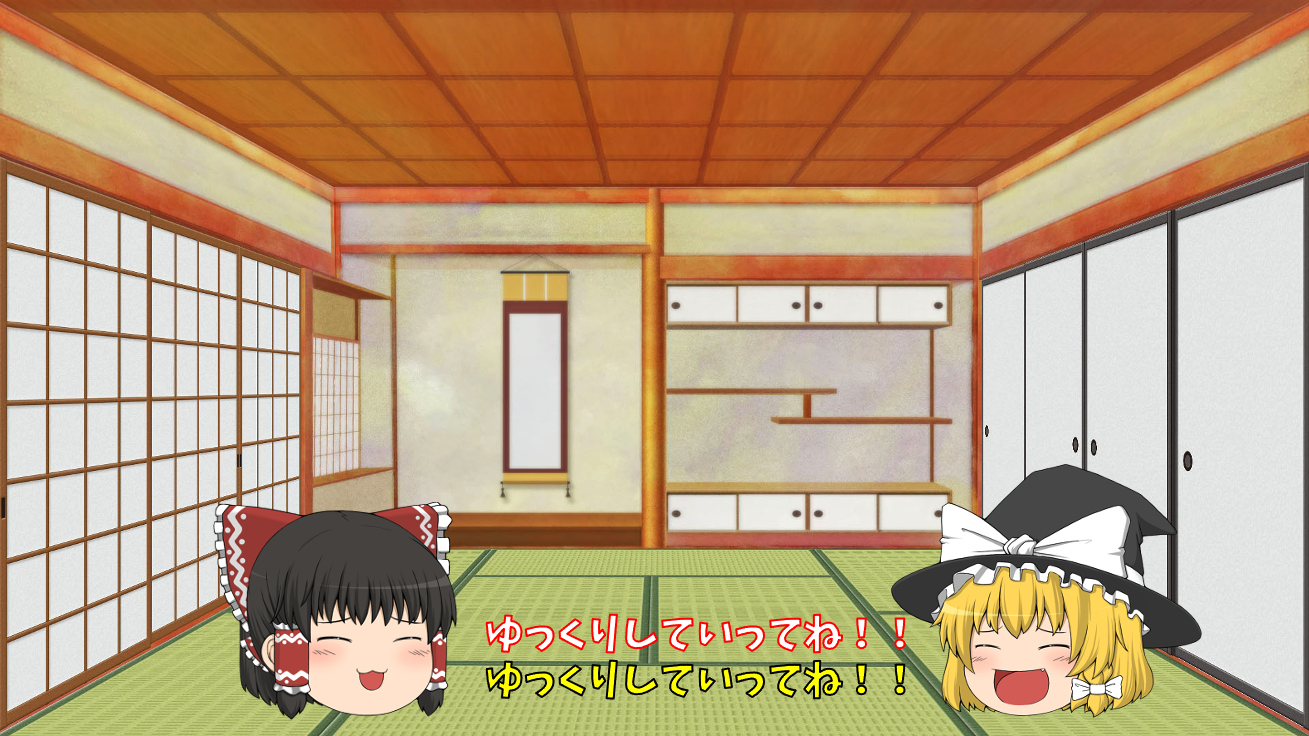
\includegraphics[width=6cm]{img-1.png}
  \caption{ゆっくりしていってね!!!}
\end{figure}
  おそらく一度は見たことがあると思うのですが、こちらは「ゆっくり」と呼ばれる謎の人頭の饅頭型キャラクターです。現在、YouTube他多くのインターネット上のプラットフォームのあらゆる界隈に進出しており、「ゆっくり実況」「ゆっくり解説」「ゆっくり茶番劇」などの多彩な動画ジャンルを産んでいます。Googleで、「ゆっくり」のワードで動画検索をかけると、その数は約 35,200,000 件にも及びます。\\
実は、ゆっくりの誕生にもPC-98が深く関わっているのです。

ゆっくりには元ネタがあります。「れいむ」「まりさ」「さなえ」「ようむ」などの名前が何なのか気になって調べた人も中にはいるのではないでしょうか。ゆっくりはゲーム「東方Project」に登場するキャラクターが元になったものなのです。\\
それをインターネット掲示板「2ちゃんねる」(現5ちゃんねる)上の誰かが、人頭饅頭型の霊夢・魔理沙\footnote{どちらも東方Projectのキャラクターの一人です。}が「ゆっくりしていってね!!」と喋っているAA(アスキーアート)を作ったのが始まりです。\\
そしてなんと、元ネタとなったゲーム「東方Project」は、PC-98のゲームなのです。\footnote{東方Project第1弾~第5弾までが、PC-98上で動作するように作られました。}\\
PC-98中期~後期には、それまで企業や一部の物好きな金持ちのものだったコンピュータが、一般家庭にも普及し始めました。その中で、PC-98は東方Projectをはじめとする多くのゲームや音楽などを通して、日本のサブカルチャーの発展に大きな影響を与えたのです。PCとそれに関わる大衆文化について考えるには、PC-98の歴史を知ることが不可欠、と言えるでしょう。
\part{98の何がいいの?}
\setcounter{section}{0}
さて、ここまでの文章を読んですでに読者の皆様は「早くPC-98について教えてくれよ!!!!」と期待の絶頂ではないかと邪推いたしますが、いかがでしょうか(笑)\\

...え?

\begin{screen}
「98がすごいPCだということはまあわからんでもない。でも、そんな30年以上前の骨董品をいじって何が楽しいんだ?」
\end{screen}

...わかりました!!そこまで仰るのなら存分に語って差し上げましょう!!\footnote{このように、ヲタクと呼ばれる人種に不用意にこのような質問をすると長時間拘束される割合が極めて高いという事実が報告されておりますので、ぜひともご注意ください。}

というわけで、以下に自分がPC-98をいじる理由を列挙してみました。\\
\section[short]{純国産PC}
現代のPCは、主にどこの国で作られているかご存知ですか?\\
現在は、たとえ日本のメーカーであっても設計程度しか携わっておらず、内部パーツ、組み立て含めそのほとんどは中国や台湾などの国々で製造されていることが多くなっています。\footnote{最近ではなんと海外メーカーのPCをロゴだけ置き換えて我が物顔で販売している時もあるそうです。}\\
また、PCの基本設計も、前述したようにアメリカIBM社のPC/ATと互換機を基にしています。\\
PC-98を始めとする今から30~20年前のPCは、日本のメーカーが独自に設計し、日本の工場で製造されていました。\\
PC-98はOSなど一部のソフトウェアこそMicrosoft社のもの\footnote{BASICやMS-DOS、MS-Windows(後述します)のことを指します。NECも漢字ROMやBIOSは完全自社開発ですが、SHARPのX68000シリーズのHuman68kなどOSも自社製のコンピュータもあります。}をもとにしていましたが、それでさえ自社のコンピュータで動作するように独自に改良を加えていました。\\
「日本製」って、憧れますよね。また現在のPCとは一味もふた味も扱い方が新鮮でおもしろいものです。\\
\section[short]{苦労への憧れ}
皆さんは、「インターネット老人会」というワードを知っていますか?\\
これは、インターネットの黎明期にインターネットを使い始めた人たちのことを指します。\\
彼らは、誰よりも先にインターネットというものを知り、それを使ってみて、時には問題を解決しながら、インターネットやPCを使いこなしていきました。そして、彼らがそれらの技術について知見を深め、利用者の輪を広げ、新しいものを発明してくることでインターネットは今や世界中の人々にとってなくてはならないものになっています。\\
彼らは、新しい技術に触れ、そこに無限の可能性を感じながらそれらを自分たちでいじることを楽しんでいたのです。
現在で例えるとすれば、ChatGPTや生成AIに色々な命令をしてみて、「今日はこんな事ができるようになった!!」「AIってすげえ!!」と言っている人たち、になるんでしょうか。\\
私はその先駆者たちに強く憧れを感じています。\\
新しい技術というものは、いつでも厳しい努力を必要とするものであって、それらの苦労を楽しむという姿勢は大いに尊敬するに値します。\\
PC-98を扱うのも、現代のPCの何倍も難しいものです。しかし、その苦労を実際に体験してみることで、彼らのことを追体験できるのではないか、と思っています。
便利なツールがひとつもない中でコンピュータを動かすにはコンピュータについての深い理解が必要となります。古いPCを扱うことで、現代では当たり前のように機械がやってくれることを自分でやることになりますが、それをすることでコンピュータについての理解がさらに深まると思っています。\\
\section[short]{こまけぇこたぁいいんだよ!!}
ここまで散々語らせていただきましたが、はい。もういいじゃないですか。だってPC-98かっこいいじゃないですか。(殴\\
今までの理由も後付けで、自分ももはやなぜPC-98に興味を持ち、いじりだしたかはよくわかりません。\\
でも、「好きなこと」って、そういうものだと思います。もう私はPC-98の虜です。好きでなければ、こんな長い文章を書こうとは思いません(汗)
\part{ハードの紹介}
\setcounter{section}{0}
随分と長い前置きが終わったところで...お待たせいたしました!早速PC-98についての紹介に入っていきたいと思います。
まずはハードウェアから。
\section[short]{PC-98の見つけかた}
PC-98の中でも時代やモデルによって異なる部分は多いですが、他のPCと比べて、PC-9800シリーズを見分けるための特徴がいくつかあります。\\
\subsection[short]{アローライン}
PC-98と他のPCを一目で見分ける特徴のひとつに、アローラインがあります。\\
これは、全面パネルにあしらわれた紋様で、PC-98特有のデザインです。\\
変化しながらも、最終モデルやその先の後継シリーズまで継承されています。\\
\subsection[short]{起動音}
PC-98のほとんどのモデルで、電源投入時に「ピポッ」という起動音を聞くことができます。\\
これも、PC-98をアイデンティファイする要素の一つとなっています。\\
音程や音色は起動音を発するマシンで共通ですが、マシンの速度その他の要因で、音の長さが変わります。\\
よって、「ピーポー」と鳴ったり「ピポ」と鳴ったり速すぎて「ピョ」と聞こえる機種もあります。\\
\subsection[short]{キーボード}
現在一般的なAT互換機用のキーボードとは異なり、PC-98のキーボードは、キーの配置や形状が独特です。\\
\subsection[short]{モデル}
PC-98のほとんどのモデルで、正面左上に「PC-98」で始まるモデル名のロゴがあります。(後述)\\
\section[short]{機種を見分けよう 〜モデル名〜}
PCの写真を見て「98だ!」と思えるようになればまずは合格です。\\
ですが、ひとくちに 「PC-9800シリーズ」と言っても、多種多様な製品があります。これらを見分けるためには、モデル名を見ることが重要です。\\
PC-98には、ほぼずべて「PC-98」で始まるモデル名がついており、以降に続く英数字で各機種を見分けます。中では特別な愛称がついているものもあります。
\end{multicols}
\begin{figure}[H]
  \centering
  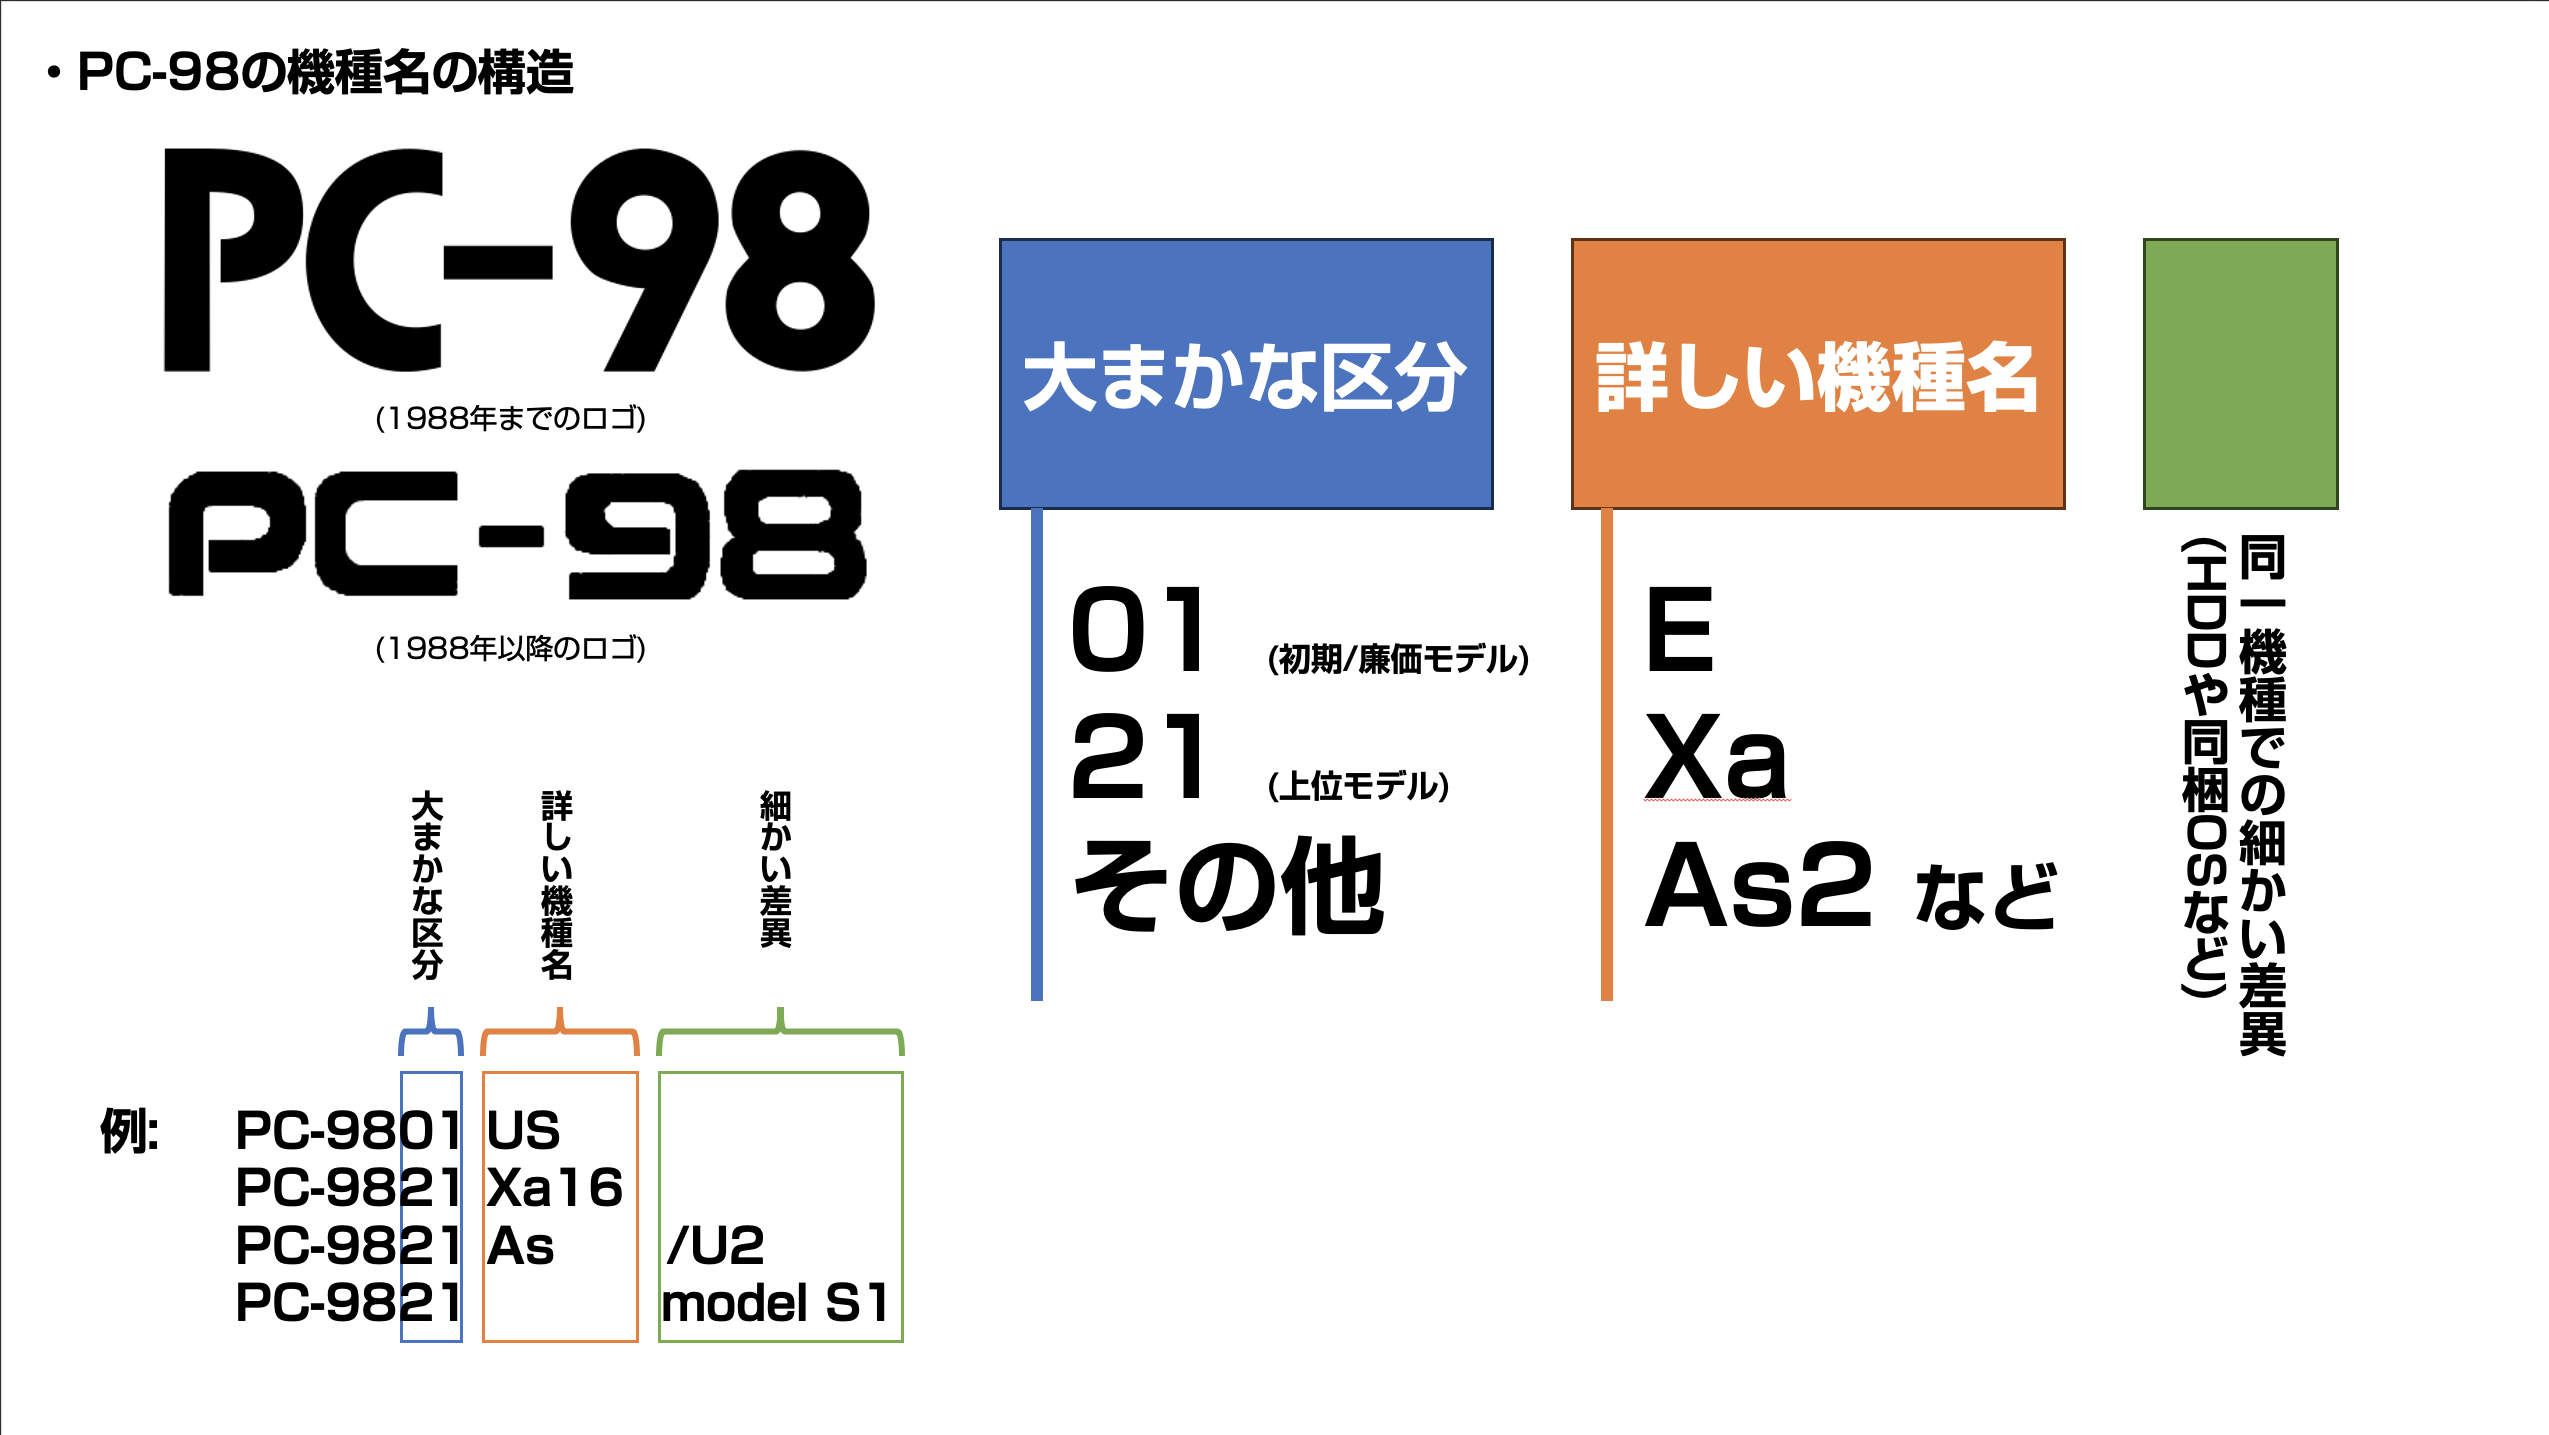
\includegraphics[width=11.5cm]{img-2.png}
  \caption{PC-98のモデル名(型番)の構造}
\end{figure}
\begin{multicols}{3}
まずPC-98の直後の「01」または「21」は大きなシリーズの差異を表します。\\
PC-9801は、PC-9800シリーズの中でも初期の製品群のことを指します。後述する「PC-9821」の登場までは、一部の特殊な製品を除いてPC-9800シリーズにはPC-9801型番しかありませんでした。\\
PC-9821は、1992年から登場したPC-9801の上位互換の製品群です。これによって、従来の「PC-9801」型番は、PC-9800シリーズの中で、廉価モデルや入門モデルの機種に付けられるようになりました。\\
その他では、PC-98LT(最初期のノートモデル)やPC-98XA(グラフィックス特化モデル)など、一部の特殊モデルには「PC-98」以下に01や21がつかない物があります\footnote{このような特殊モデルは、PC-9801を基本設計としながらも独自機能を多く搭載していたため、「PC-98」の名前を冠していながらも他機種との互換性が低く売上が伸び悩む傾向にあったようです。}。
次にその次に続く英数字は、その機種の詳細なモデルを指します。\\
モデルの中では、似た特徴を持つものに相性がつけられていることもあります。\\
モデル名の中でも有名なものを紹介します。\\
\subsection{最初期モデル}
1982年に発売された初期モデルから84年までのモデルを見ていきましょう。
PC-9800シリーズは、1982年にそれまでのPC-8800シリーズの後継・上位シリーズとして主にビジネス用途を想定しながら始まりました。
この頃のモデルはシリーズの出始めということで、手探りしながらPC-98の基本を形作ります。
CPUはIntel 8086互換のNEC製\ruby{μ}{ミュー}PD8086を搭載しました。
基本的なグラフィックス機能として、図形描画機能や拡大表示機能などをもち最大640ドット×400ドット8色表示に対応したチップ(GDC)\footnote{Graphic Display Controller}を搭載しています。
アローラインは茶色で窪みをつけて直線的に引かれます。太い部分が以後の機種は大体が左なのですが、この頃のモデルのみ右側が太くなっています。
\begin{table}[H]
  \centering
    \begin{tabular}{ll}
        {\bf PC-9801} & 伝説の初代モデル\\ \hline
        発売日 & 1982年10月13日\\
        標準価格 & 298000円\\
        CPU & NEC μPD8086 5MHz\\
        メモリ & 128KB\\
        補助記憶 & 内蔵なし\\
        内蔵音源 & BEEP音のみ\\
        \end{tabular}
\end{table}
シリーズ最初のモデルです。\\
8086搭載・GDC搭載など、後のモデルに引き継がれる最も基本的な機能が搭載されています。\\
ドライブが搭載されていないため、情報を保存するためには別途外付けで8インチまたは5インチFDD、もしくはテープレコーダなどを増設する必要がありました。\\
日本語表示機能は標準で半角カナのみであり、漢字などを表示するためには別途拡張ROMを増設する必要がありました。\\
これに続けて、CPUを若干速度向上させた上で漢字ROMとFDDを内蔵させたPC-9801F、価格を抑えたPC-9801E\footnote{{\bf E}conomyだと思われます}などが発売されました。\\
\end{multicols}
\begin{figure}[H]
  \centering
  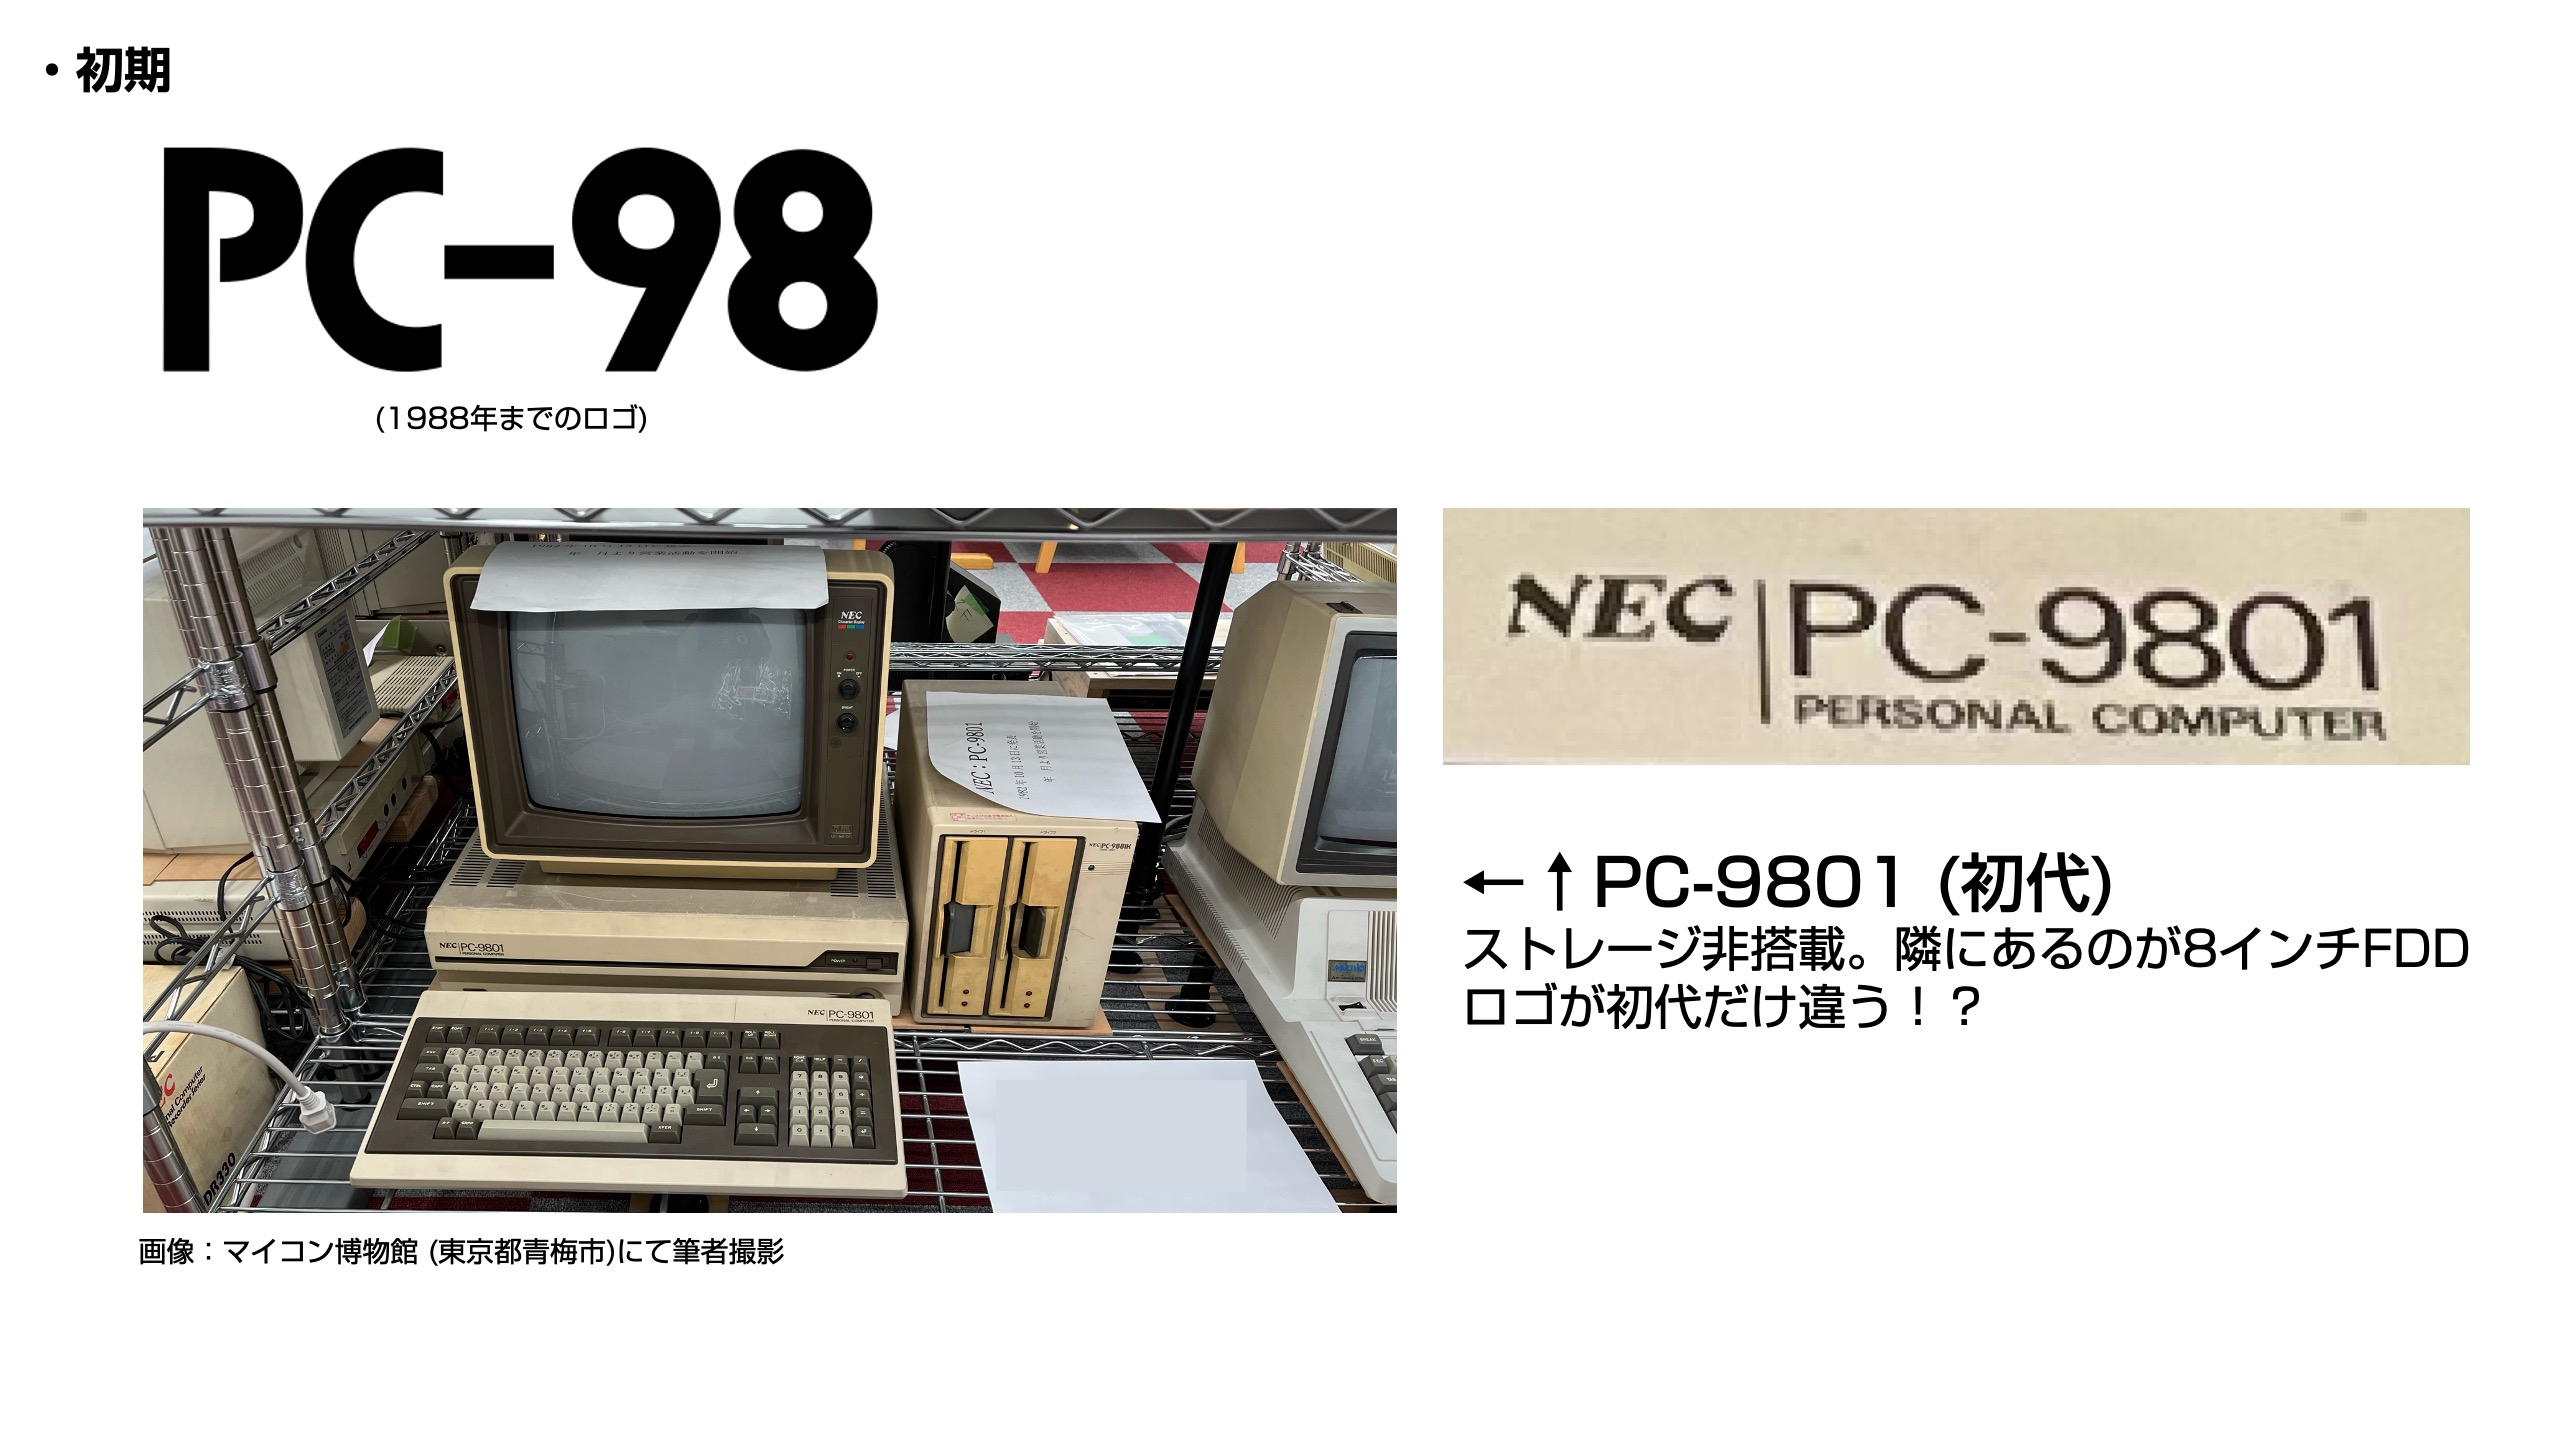
\includegraphics[width=12.5cm]{img-7.jpg}
  \caption{PC-9801}
\end{figure}
\begin{multicols}{3}
\subsection{前期モデル}
1985年から1988年までのモデルを見ていきましょう。\\
この頃のモデルは、PC-98の基本的な機能が固まり、多くのユーザーに受け入れられるようになりました。\\
CPUはIntel 8086の互換性を保ちながら速度を向上させたNEC製V30を搭載しました。\\
GRCG\footnote{Graphic Charger,GCとも}というチップの追加によりグラフィックス機能が大幅に強化され、処理の高速化と出力方式の追加によって4096色中16色同時発色表示を実現しました。\\
普及するにつれて家庭用途にも使われるようになり、FM音源を搭載したモデルも登場しました。\\
アローラインは茶色で窪みをつけて直線的に引かれます。それまでのモデルと異なり、太い部分が左側になります。また、アローライン周辺に排熱用のスリットが設けられています。\\
\begin{table}[H]
  \centering
    \begin{tabular}{ll}
        {\bf PC-9801VM} & 黄金期の始まり\tablefootnote{以下はメジャーなVM2のスペックです}\\ \hline
        モデル & 0/2/4(前期)\\
        発売日 & 1985年7月\\
        標準価格 & 415000円\\
        CPU & NEC V30 10MHz\\
        メモリ & 384KB\\
        補助記憶 & 5インチFDD2基\tablefootnote{2HD/2DD自動切換機能搭載}\\
        内蔵音源 & BEEP音のみ\\
        \end{tabular}
\end{table}
PC-98一強時代を築くきっかけとなったモデルです。\\
PC-9801Fと比較して約2倍高速と言われる基本性能と幅広い拡張性から、長く使えるとして多くのユーザーに支持され、VM2は20万台を売り上げました。\\
FDD非搭載のVM0と5インチFDD2基搭載のVM2が最初に発売されてから、9月にはついにHDD\footnote{SASI接続、20MB}を搭載したVM4も登場しました。\\
VMでは16色表示をするためには別売りの拡張カードを追加する必要がありました。\\
\begin{table}[H]
  \centering
    \begin{tabular}{ll}
        {\bf PC-9801UV}2 & コンパクト+高性能\\ \hline
        発売日 & 1986年7月\\
        標準価格 & 318000円\\
        CPU & NEC V30 10MHz\\
        メモリ & 384KB\\
        補助記憶 & 3.5インチFDD2基\\
        内蔵音源 & FM音源\tablefootnote{PC-9801-26ボード相当。FM音源3和音+SSG音源3和音}\\
        \end{tabular}
\end{table}
シリーズ初のFM音源搭載モデルです。\\
少し前に発売されたPC-9801Uは3.5インチFDDを搭載しながらも、VMと比較して貧弱なスペックでした。\\
UV2はVMと基本スペックは同等、さらにFM音源も搭載しているほか、グラフィックスも標準で16色表示が可能で、VMと一緒に長く活躍しました。\\
この後、VM、UV共にメモリ増強などを行ったマイナーチェンジモデルのVM21\footnote{VM21は起動音が鳴る初のマシンとのことです}、UV21などが発売されました。\\
\end{multicols}
\begin{figure}[H]
  \centering
  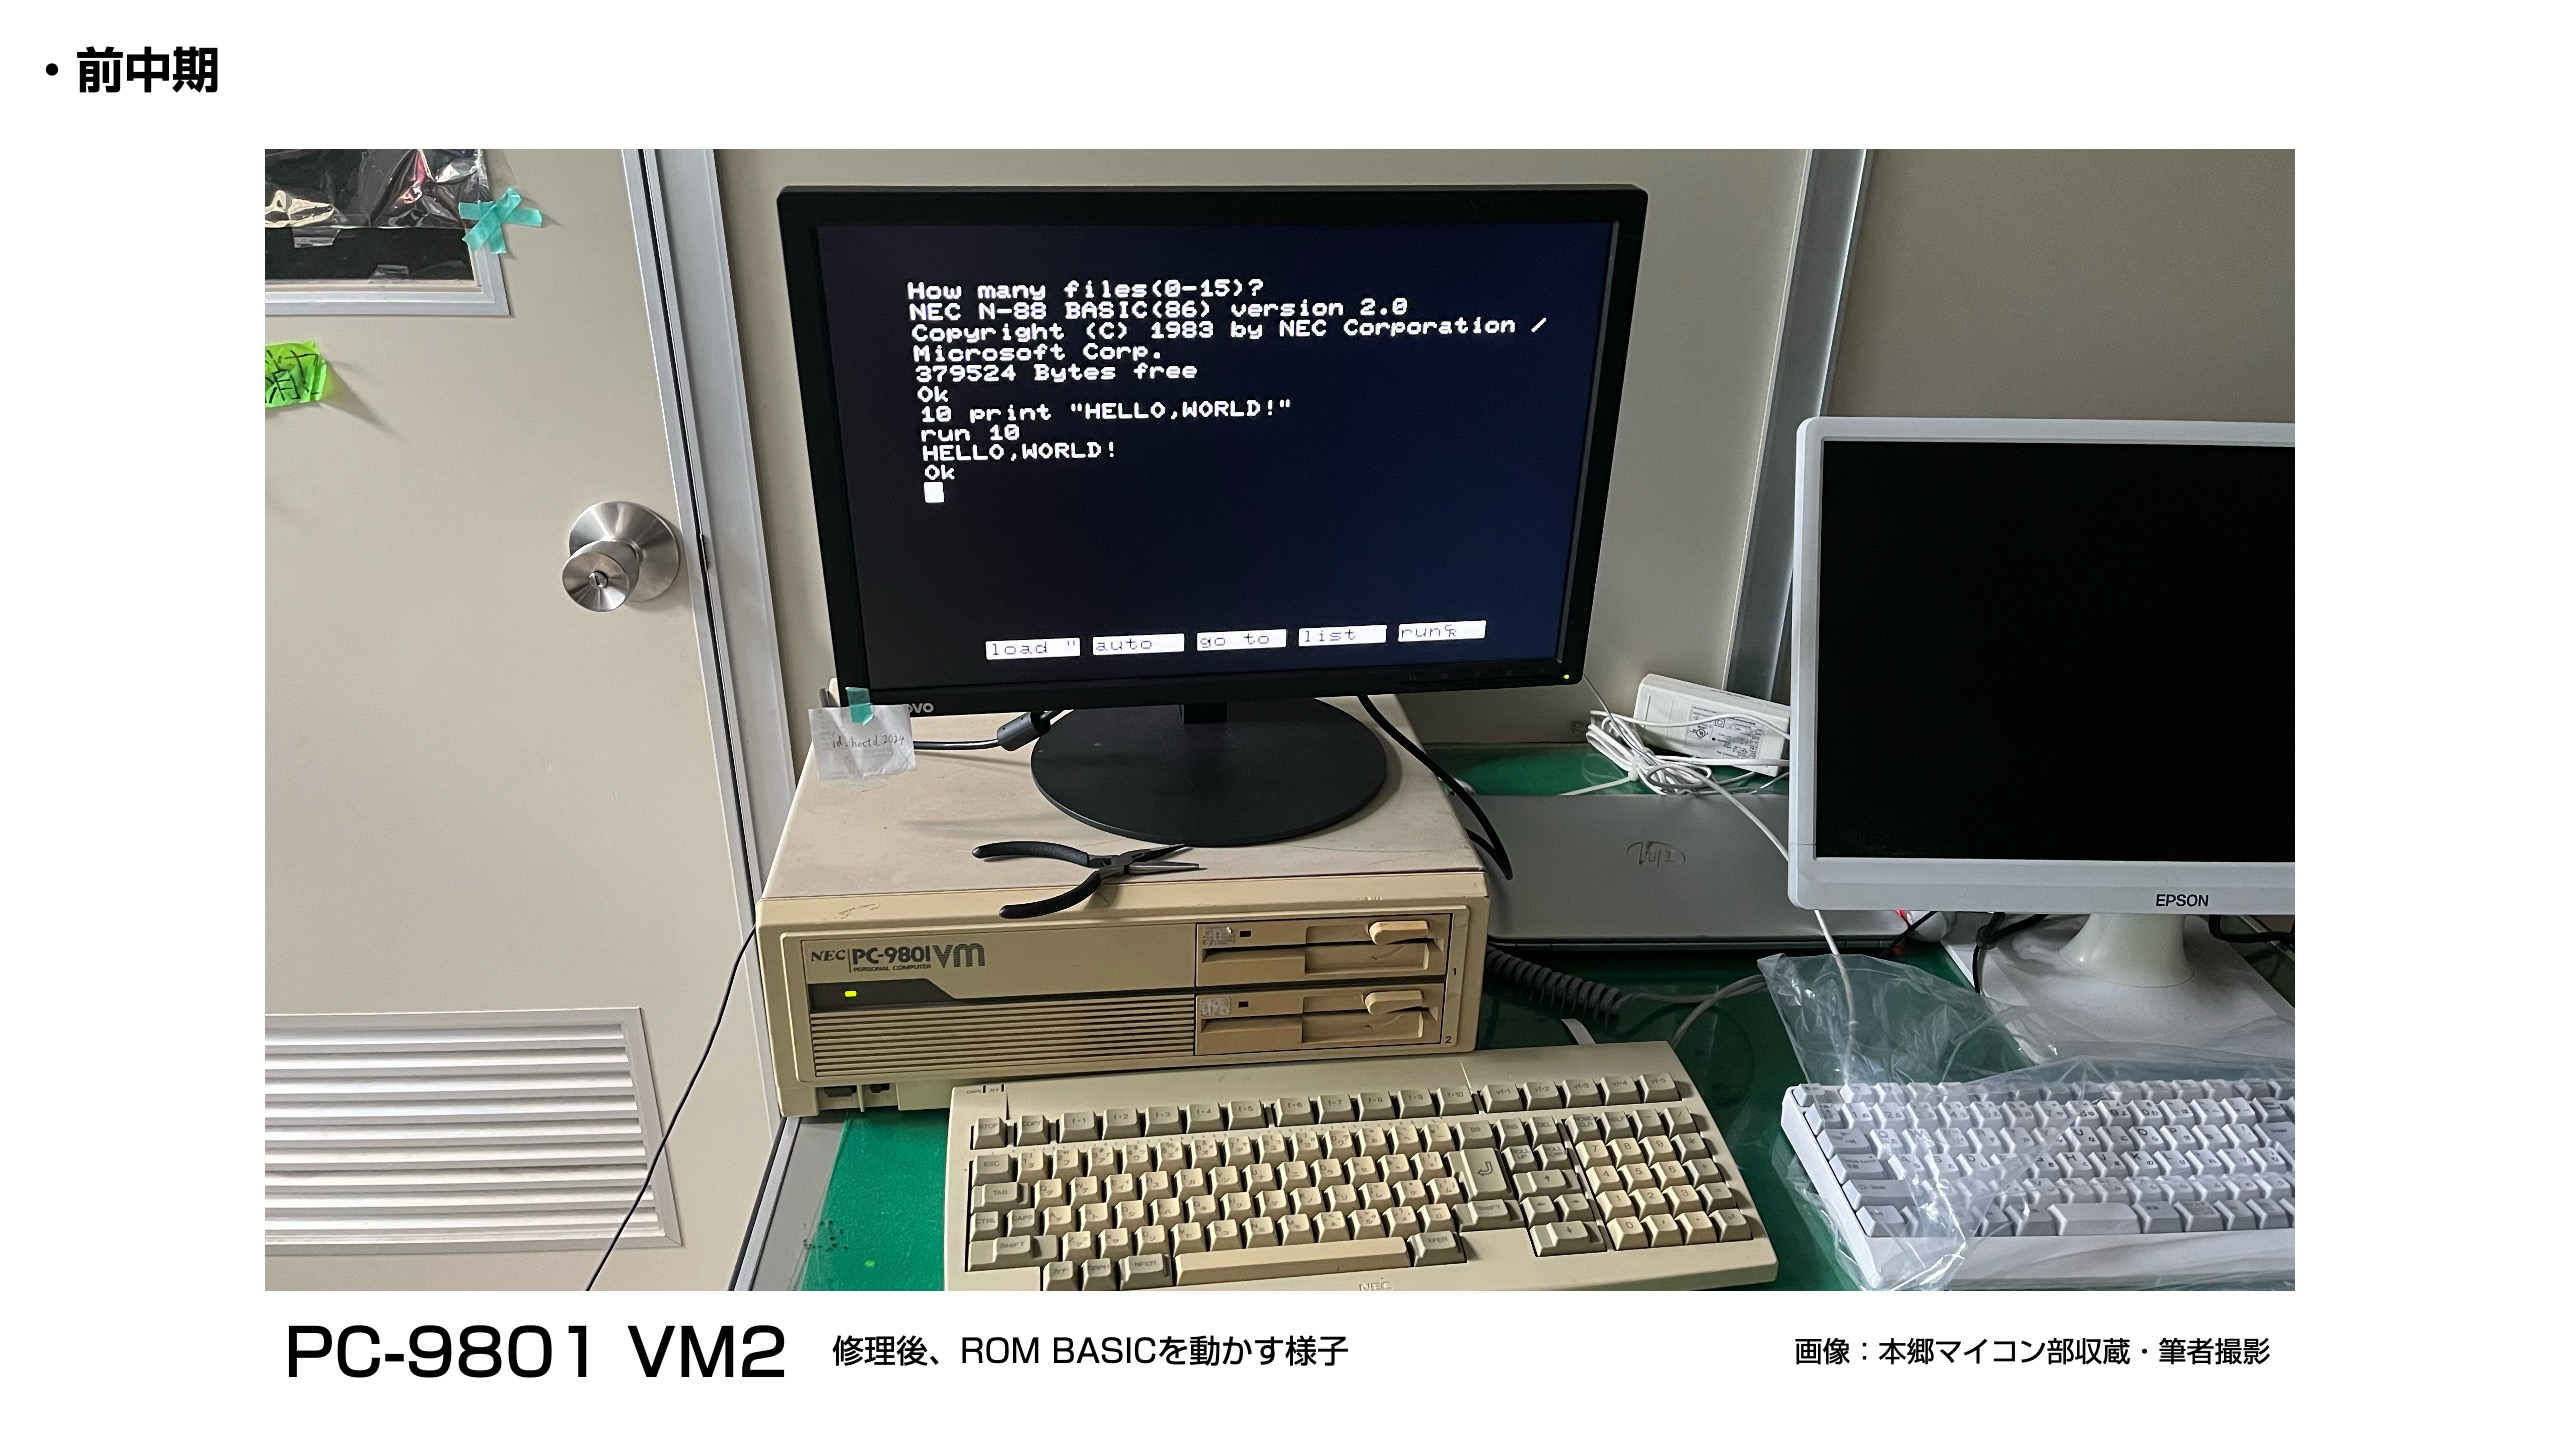
\includegraphics[width=12cm]{img-8.jpg}
  \caption{PC-9801 VM2}
\end{figure}
\begin{multicols}{3}
\subsection{中期モデル}
80年代後半から90年代初頭にかけてのモデルを見ていきましょう。\\
この頃は、MS-DOSの普及とハードウェアの高性能化によって、PC-98が絶頂期を迎えます。\\
CPU/グラフィックの性能向上、ノートPCの登場、本格的に家庭用途を意識したモデルの登場など、多くの意欲的なモデルが登場しました。\\
CPUは8086の順当進化モデル、80286や80386(i386)が搭載されました。初めの方は、V30にあり、286になかった機能を利用したソフトウェアのために、両方のCPUを搭載して、全面のスイッチでどちらを使用するか切り替えられるモデル(!?)が発売されました。\\
グラフィックは、GRCG互換で、さまざまな速度向上を行なったEGC\footnote{Enhanced Graphic Charger}が搭載されました。またクロックを従来の2.5MHzと5Mhzから選べるようになったGDC x 2 + EGCの構成が事実上の標準となり、一つのチップに集積されるなど形を変えながらも最終モデルまで継続することになります。\\

\begin{itembox}[l]{"国民機"EPSON PCシリーズ}
1987年、セイコーエプソン(EPSON)からPC-98互換機の「PC-286 model 1〜4」が発表されました。この互換機は一度NECに著作権の侵害であるとして訴訟を起こされ、販売されないままモデルチェンジを行い1987年4月24日、PC-286 model0が発売されました。この後、EPSON PCシリーズは本家PC-98と価格面、性能面、著作権面でNECと競合していくことになります。\\
\end{itembox}
\end{multicols}
\begin{figure}[H]
  \centering
  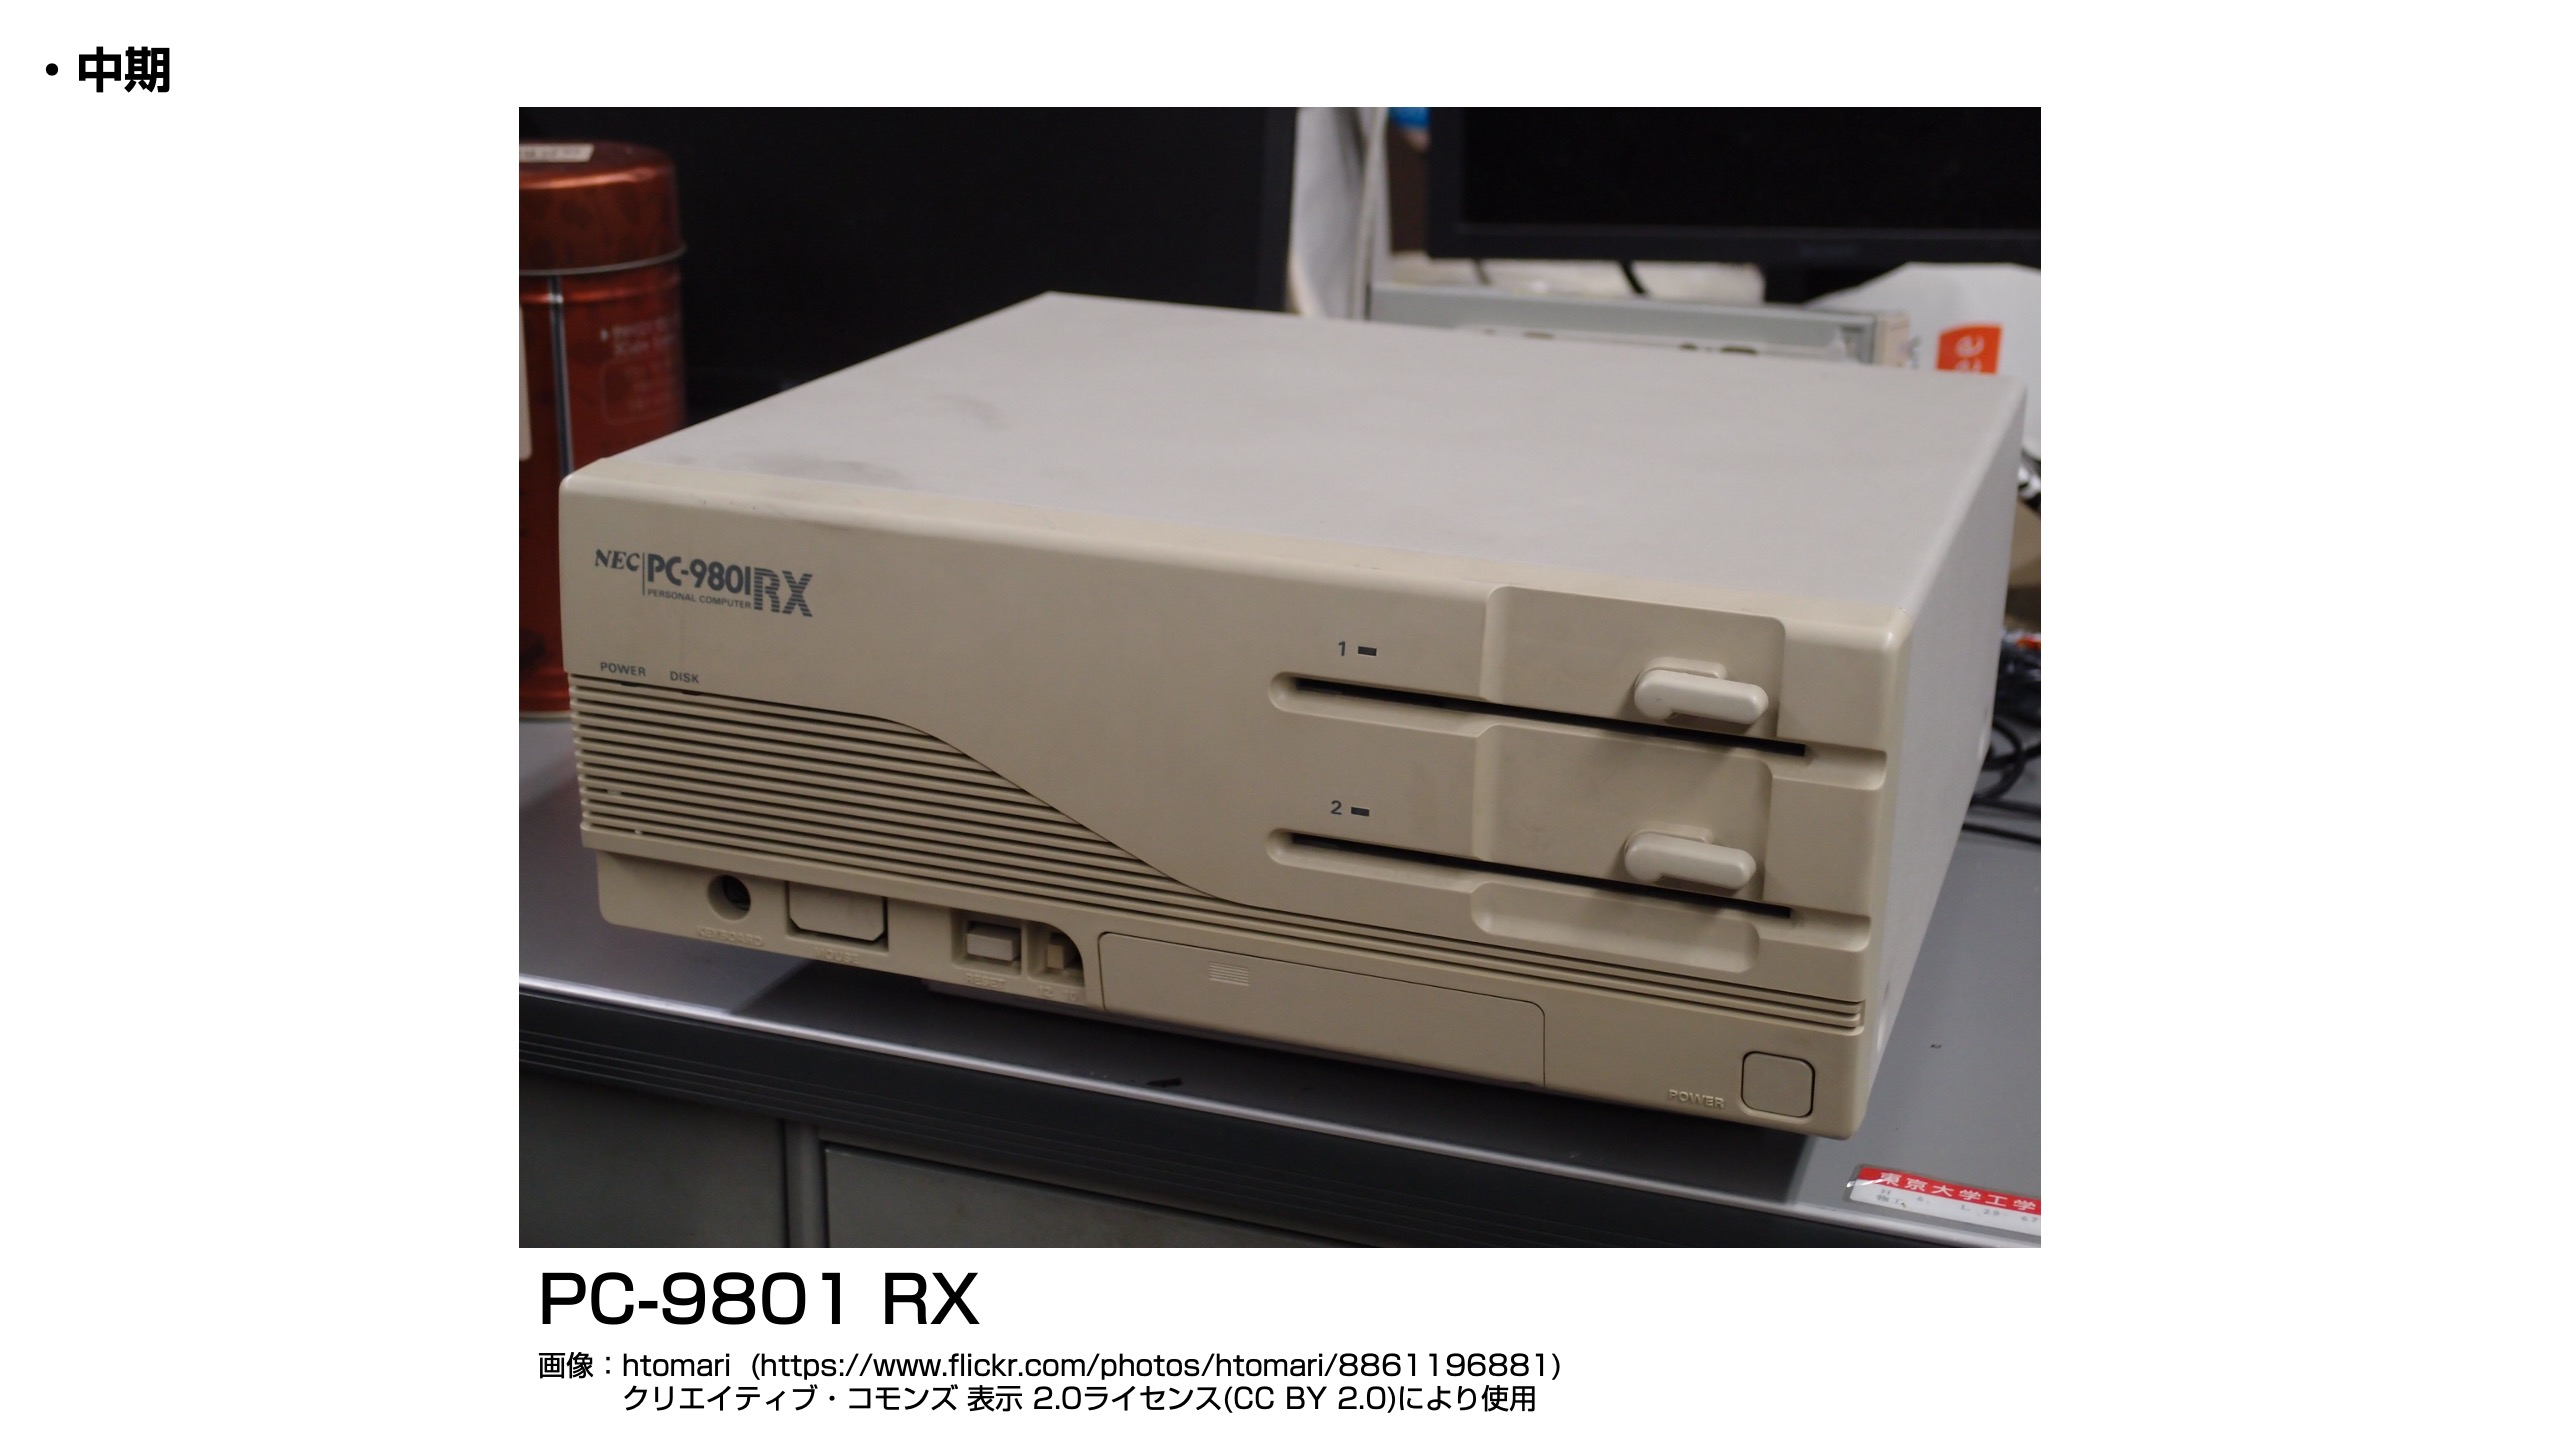
\includegraphics[width=12cm]{img-9.jpg}
  \caption{PC-9801 RX}
\end{figure}
\begin{multicols}{3}
\begin{table}[H]
  \centering
    \begin{tabular}{ll}
        {\bf PC-9801 RX} & 内部もデザインも一新した新・標準機\\ \hline
        モデル & 2/4(前期)/21/51(後期)\\
        発売日 & 1988年9月\\
        標準価格 & 398000円(2)/566000円(4)
        CPU & NEC V30 8MHz+Intel 80286 12Mhz\\
        メモリ & 640KB\\
        補助記憶 & 5インチFDD2基\\
        内蔵音源 & BEEP音のみ\\
        \end{tabular}
\end{table}
%PC-9821 As、Ap、Ae、An等Aがつくモデル...\\
%\ruby{MATE}{メイト} A シリーズ\\
%PC-9821 Cb、Cx、Ct、Cu等Cがつくモデル...\\
%98\ruby{MULTi}{マルチ} \ruby{CanBe}{キャンビー} シリーズ\\
%PC-9821 V13、V16、V20等Vがつくモデル...\\
%\ruby{VARUESTAR}{バリュースター} シリーズ

\part{PC-98のソフトたち}
\setcounter{section}{0}
ハードを見終わったところで、次はソフトウェアについて見ていきましょう。\\
ソフトウェアとは、コンピュータ(ハードウェア)が実行するデータのことです。\\
ゲームで例えると、「Nintendo Switch」はハードウェア、そこで実行されている「スーパーマリオブラザーズ」はソフトウェア、といった感じです。
\section[short]{ソフトウェアの区分}
PC-98に限らず、コンピュータには「基本ソフトウェア」「応用ソフトウェア」という区分があります。\\
この先の便宜上解説をしておこうと思います。\\
\begin{figure}[H]
  \centering
  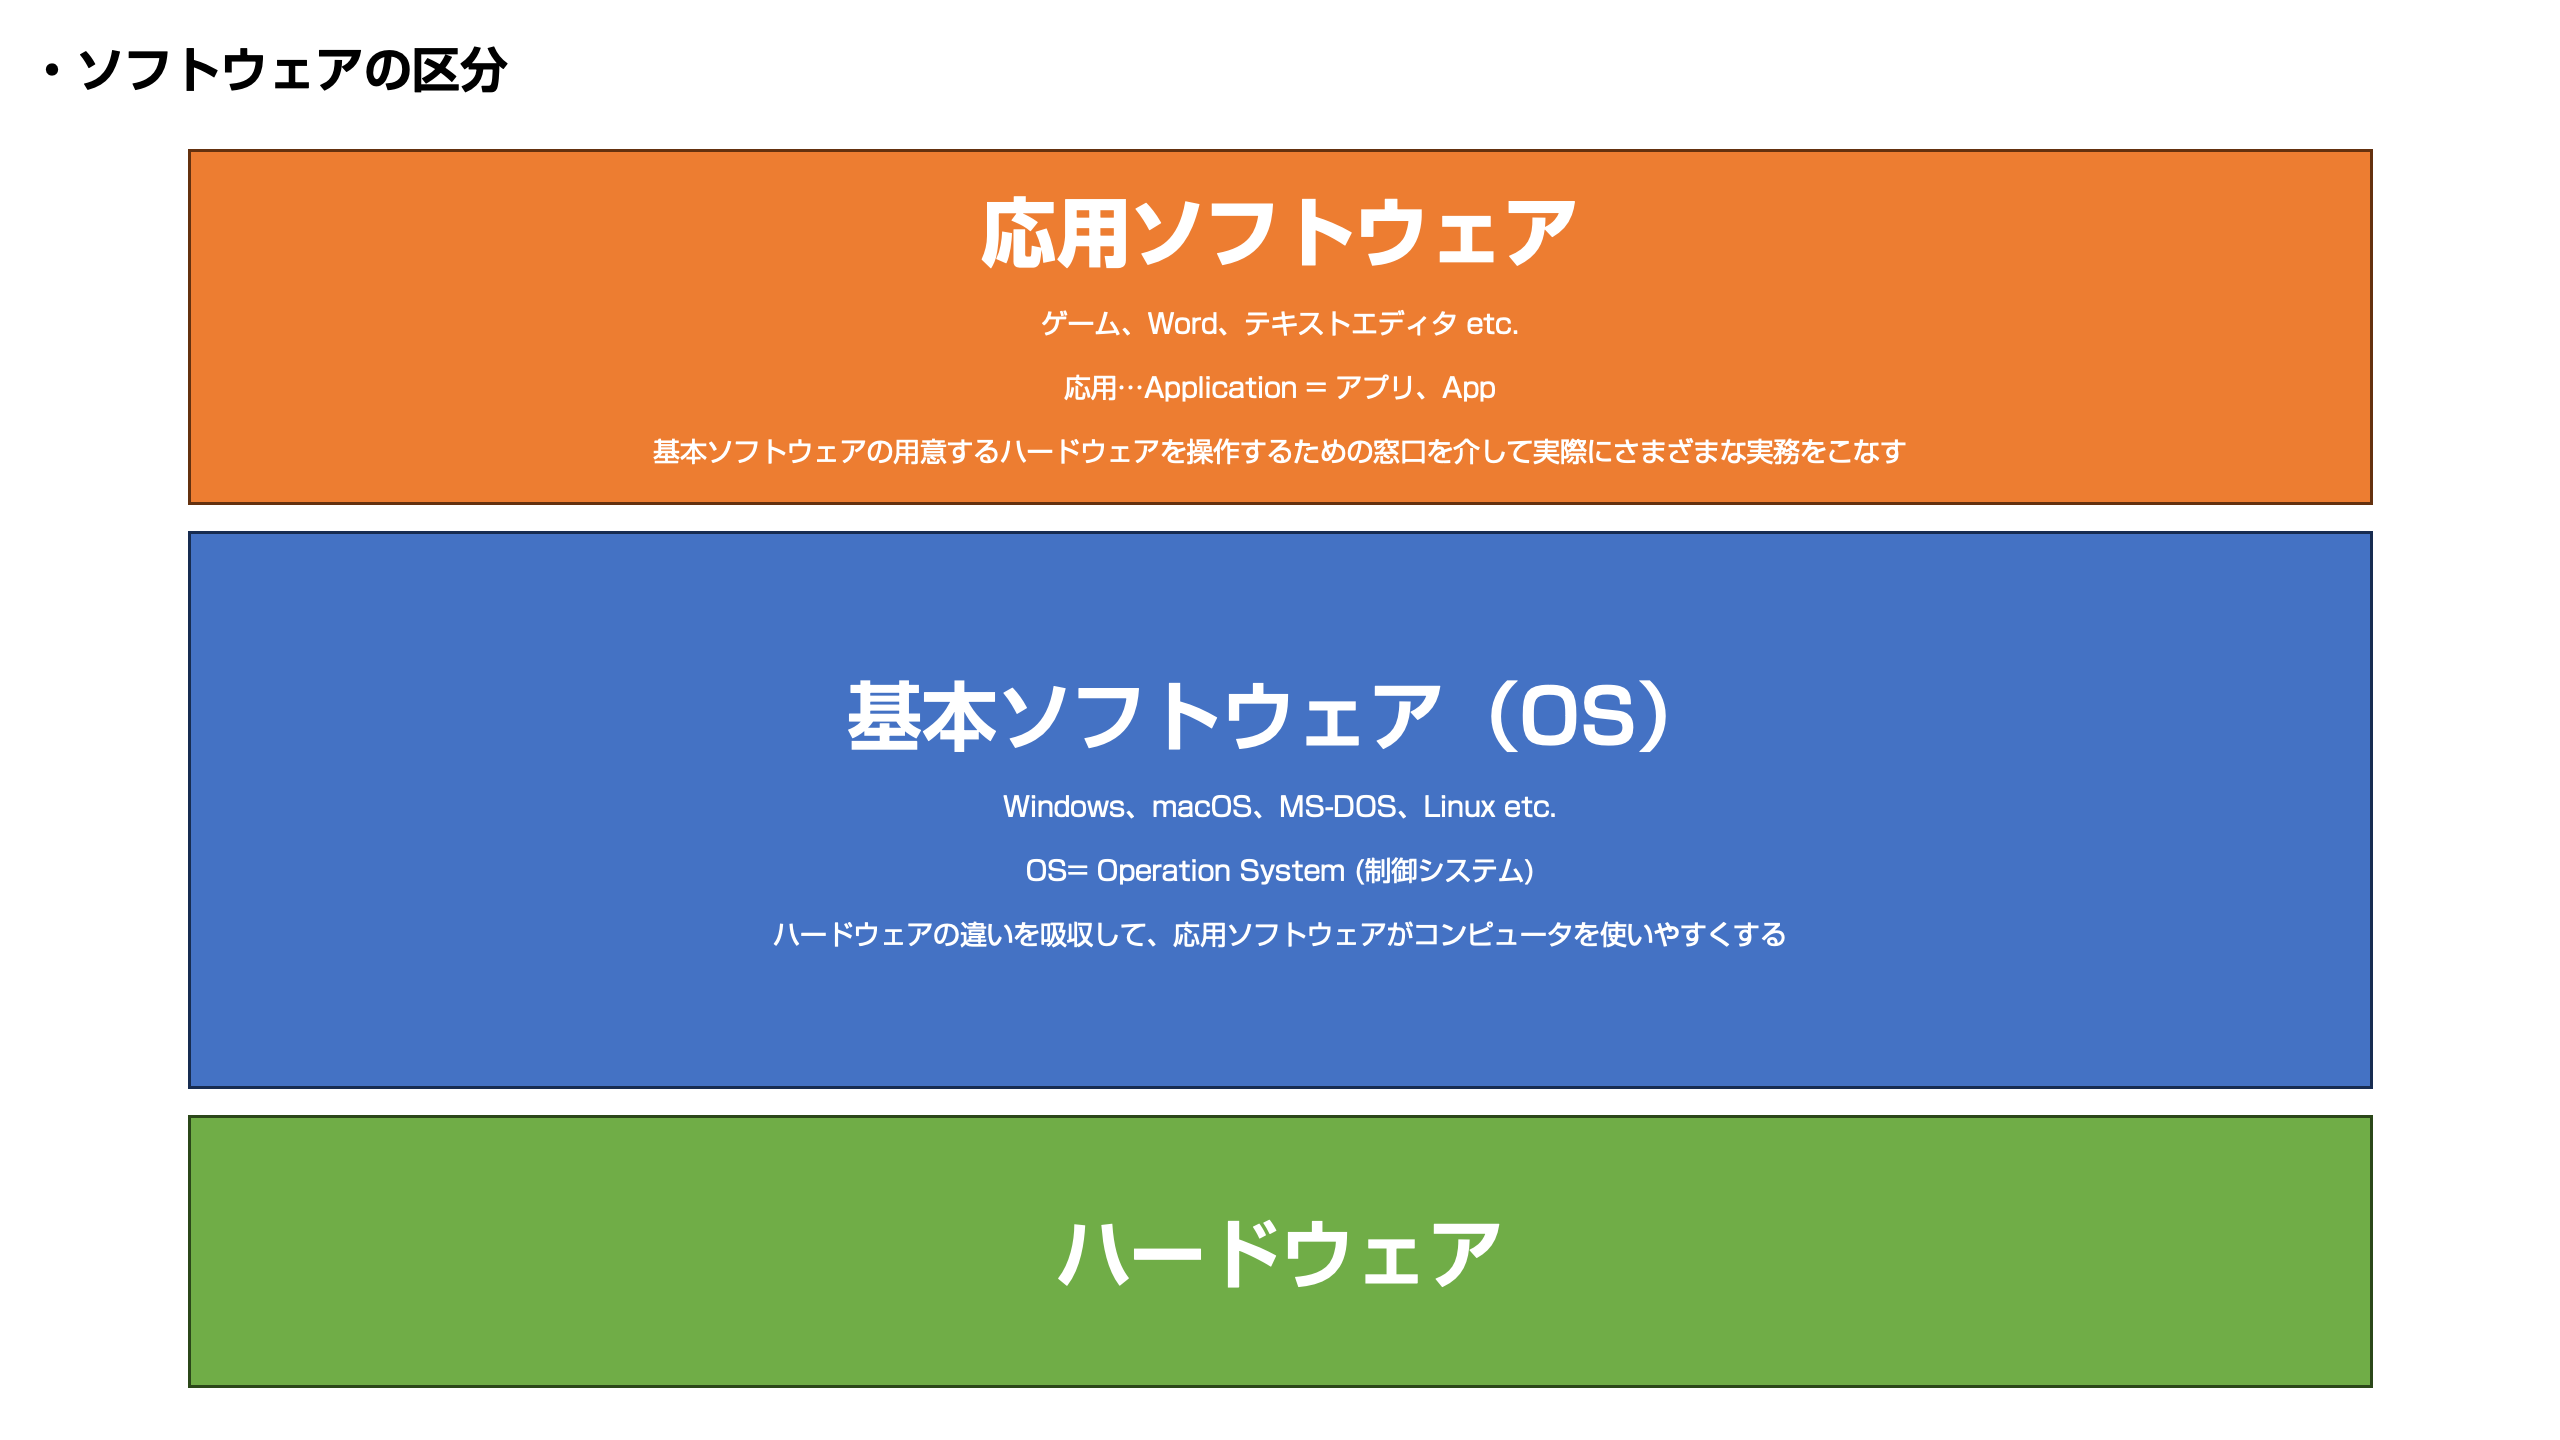
\includegraphics[width=5cm]{img-6.png}
  \caption{ソフトウェアの区分}
\end{figure}
\begin{enumerate}
  {\bf \item 基本ソフトウェア \\}
  基本ソフトウェアとは、コンピュータの基本的な機能を提供するソフトウェアのことです。\\
  コンピュータは、機種や構成によりさまざまに異なります。それを吸収して、応用ソフトウェアが動作するための窓口を提供します。\\
  たとえば、キーボードの接続方式やそのキー配列は環境により異なりますが、基本ソフトウェアのはたらきにより応用ソフトウェアは単に「何のキーが押されたのか?」という情報を受け取ることができるようになっています。\\
  iOSやWindows、AndroidなどのOS(オペレーティングシステム)\footnote{広義の基本ソフトウェアです。ここでは分かりやすくするために基本ソフトウェア=OSという形で解説しています。}を思い浮かべるとわかりやすいでしょう。\\
  PC-98の時代でも、その進歩に応じて、基本ソフトウェアは進化していきました。\\

  {\bf \item 応用ソフトウェア \\}
  応用ソフトウェアとは、OSが提供するコンピュータの基本的な機能\footnote{API(Application Programming Interface)と言います。}を利用して、特定の目的に応じた機能を提供するソフトウェアのことです。\\
  たとえば、表計算ソフトや画像編集ソフト、ゲームなどがこれに当たります。\\
\end{enumerate}

\section[short]{PC-98ソフトウェア列伝}
PC-98には、多くのソフトウェアがあります。\\
OSは技術の進化を、ゲームなどは文化の変容を、ビジネスソフトは社会の変化を、それぞれよく反映したものとなっています。\\
\subsection[short]{OS}
PC-98の時代をOSごとに区切ると、大きく分けて以下のようになります。\\
\begin{figure}[H]
  \centering
  \begin{tabular}{ll}
    普及年代 & OS\\ \hline
    1982 & $\rm{N_{88}-BASIC (86)}$\footnote{厳密にはOSではありませんが、便宜上そうしておきます。}\\
    1985 & MS-DOS\\
    1995 & MS-Windows\\
  \end{tabular}
  \caption{PC-98のOSの系譜}
\end{figure}
  いかがでしょうか。\\
\part{ふろく:PC-98用語集}
付録として、PC-98を構成するパーツについてご紹介します。とはいっても、その大部分は現代のPCと同じです。\\
最新のPCの情報も併記しておりますので、その違いを楽しんでいただければと思います。\\
ここでは各パーツの概要にのみ触れています。興味が湧くパーツがあれば、ぜひとも調べてみてください。\\
\begin{enumerate}
  {\bf  \item CPU\\}
  \begin{figure}[H]
    \centering
    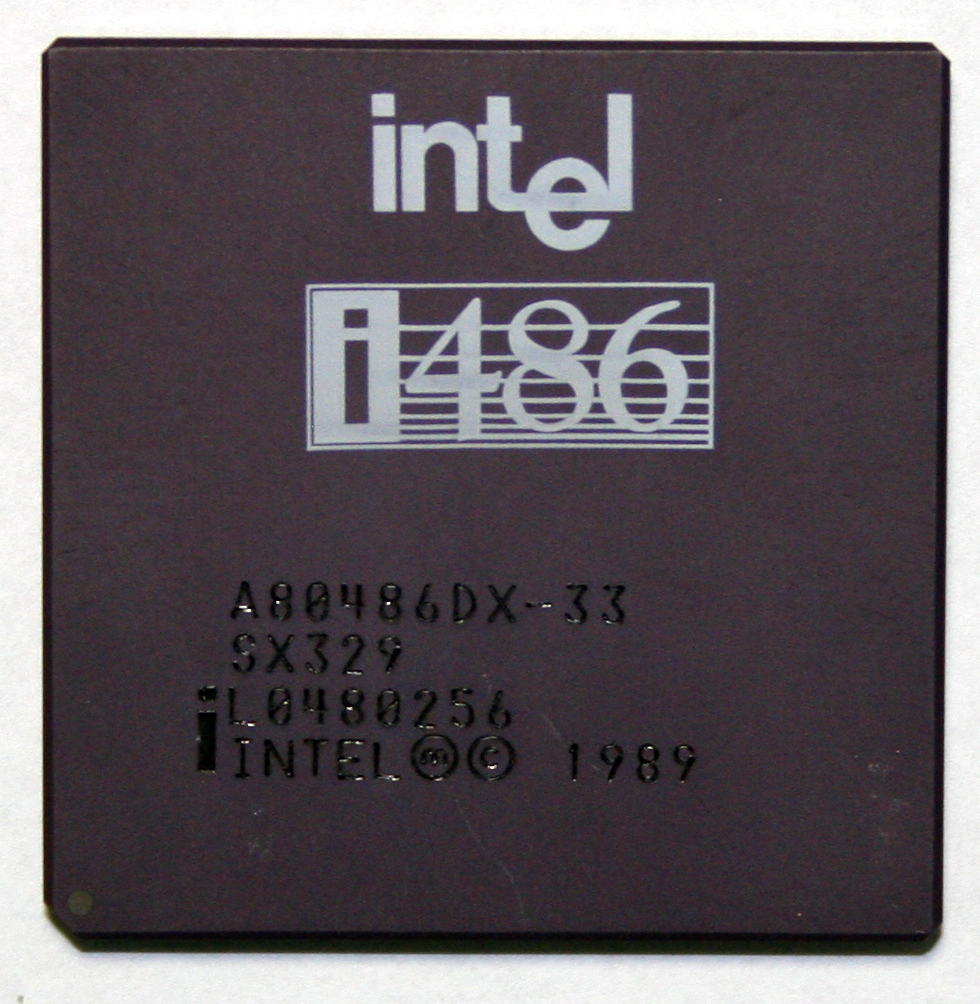
\includegraphics[width=5cm]{img-5.jpg}
    \caption{Intel i486DX}
  \end{figure}
CPU(Central Processing Unit,中央処理装置)は、コンピュータのまさにメインとなる、頭脳にあたる部分です。コンピュータの命令を解釈し、実行します。\\
PC-98には、主にIntel社製の「Intel 8086」とその後継および互換CPUが搭載されています。\footnote{初期のPC-98では、8086と完全な互換性を保つために、8086とより性能のよいCPUを両方搭載し、スイッチで切り替えができる機種もありました。}\\
現在のIntel社のCPUはほぼすべてIntel 8086の上位互換製品\footnote{ちなみに、$\rm{N_{88}-BASIC (86)}$の「86」は、NECが販売していた別機種、PC-8800シリーズに搭載のBASICを、8086用に移植したという意味です!}です。\\
CPUの速さは、そのCPUが一秒間に何回命令を実行できるかを表す「クロック周波数」で表されます。\\
現在のCPUは早いもので6GHz(1秒間に600億回)以上のクロック周波数を持っていますが、PC-98のCPUは5MHz(1秒間に500万回程度)から、早いものでも300MHzまででした。\\
こうして数字にしてみると、現代のCPUの方が圧倒的に早く、技術の進歩を感じさせられます。
今でこそ「遅い」と言えますが、当時からしてみれば100MHzを超えるCPUは高性能、300MHzなどは何でもできるスーパーマシンという認識だったのでしょう。\\
\begin{itembox}[l]{主なCPU}
  \begin{itemize}
    \item Intel 8086
    \item NEC V30
    \item Intel 80286
    \item Intel 80386
    \item Intel i486
    \item Intel Pentium
  \end{itemize}
\end{itembox}
\begin{itembox}[l]{下駄?ODP?}
とくに9821登場以降のPC-98のCPU関連の話には、「下駄」「ODP」という単語が時折登場します。\\
どちらも、性能向上を目的に元々搭載されていたCPUをなんらかの形で強化するものです。\\
下駄は、既存のCPUの上にから装着したり、ソケットに追加の部品を差し込むことで、市販のより性能の高いCPUを搭載できるようにしたり、既存のCPUのクロック周波数を上げることができるものです。\\
ユーザー有志の改造によるものもあれば、メルコ(現バッファロー)など、周辺機器メーカー製のものもありましたが、大抵メーカーのサポート対象外であることが多かったようです。\\
ODP(OverDrive Processor)は、Intelが公式に開発・販売したCPUのグレードアップキットです。\\
対通常のCPUソケットとは別にODPソケットが搭載されている対応PCに対して、ODPを差し込むことでCPUをグレードアップできます。\\
\end{itembox}

  {\bf  \item メモリ(RAM)\\}
  メモリは、コンピュータが実行するプログラムやデータを一時的に保存する部分です。\\
  一時的に電気を貯めることのできる電子部品であるコンデンサを使って、情報を記憶します。\\
  その特性上、電源を切ると情報が消えてしまいますが、その代わり読み書きはハードディスクより高速に行うことができます。\\
  現在のPCでは、一般的にDIMMというメモリ(規格によりDDR4、DDR5という呼び方が一般的)が使われていますが、PC-98ではSIMMというメモリが一般に使われていました。\footnote{一部の末期のPC-9821ではDIMMが使えるものがあったようです。}\\
  DIMMとSIMMの違いを簡単にいうと、SIMMが端子の両面とも同じ信号が流れていたのに対して、DIMMは片面ずつ異なる信号を流せるようになりました。つまり、DIMMはSIMMの2倍の情報をやり取りできるようになったということです。\\
  最近では8GBのメモリを搭載したPCがだんだん少なくなり、16GBが一般的になりつつありますが、PC-98では基本のメモリ640KB(0.00064GB)から始まり、拡張しても512MBなどがせいぜいといったところでした。しかも、増設しすぎると(プログラムがそこまでメモリがあることを想定していないために)プログラム側が誤動作する、ということもあったそうです。\\
  {\bf  \item フロッピーディスク(FDD)\\}
  \begin{figure}[H]
    \centering
    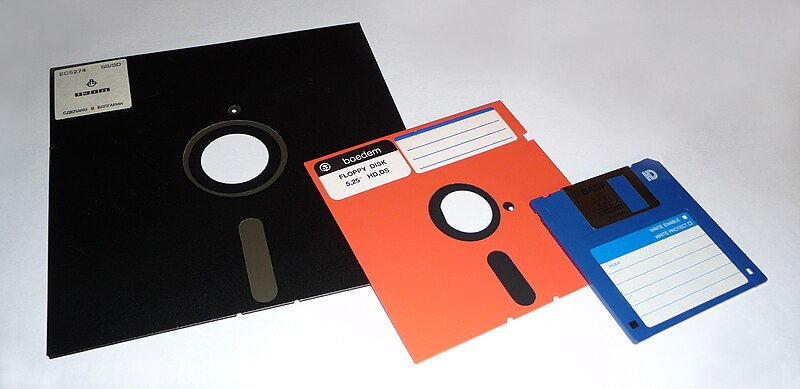
\includegraphics[width=5cm]{img-3.jpg}
    \caption{フロッピーディスク}
  \end{figure}
  フロッピーディスクは、コンピュータが実行するプログラムやデータを一時的に保存するメディアです。\\
  磁気を帯びさせることができる円盤を回転させ、その上に磁気ヘッドを接触させることでデータを読み書きします。\\
  名前の「フロッピー」は、英語で「ぐにゃぐにゃした」という意味の「floppy」に由来します。\\
  手軽にデータを持ち運ぶことができるメディアとして、この時代広く用いられました。\\
  欠点は、データを記録する円盤の保護が甘く少しの傷や汚れ、衝撃でデータが消えてしまうことと、読み書きが遅いこと、そして容量が小さいことです。\\
  保存できるデータの量は360KB(2DD)、720KB(2HD)、1.2MB(2HD)、最大で1.44MB(2HD)でした。\\
  カッコ内の英数字は、フロッピーディスクへのデータの書き込み方法の種類を表します。\\
  たとえば、2HDは両面高密度という意味で、ディスクの面裏それぞれに2倍のデータを書き込める、ということです。\\
  フロッピーディスクは、8インチ、5インチ(ミニフロッピー)、3.5インチ(マイクロフロッピー)の3種類がありました。\footnote{他にも多種多様なフロッピーのサイズが考案されましたが、定着したのは主にこの三種類のみです。}\\
  3.5インチフロッピーは、日本の大手メーカーであるソニーが開発したもので、現在でもフロッピーディスクのイメージとして定着しています。\\
  PC-98では、最初期の数モデルを除きすべての機種でフロッピーディスクドライブを搭載しています。\\
  最初期は外付けの8インチドライブ、初期から中期は内蔵の5インチドライブ、中期から末期は内蔵の3.5インチドライブが主流でした。\\
  現代ではフロッピーを実際に目にすることはほとんどなくなりましたが、長らくデータの持ち運び方法の主流であったために、PCソフトの保存アイコンに用いられたり、公官庁や金融機関ではいまだにフロッピーを使用する機器があるなどして問題になっていたりします。
  {\bf  \item ハードディスク(HDD)\\}
  ハードディスクは、コンピュータが実行するプログラムやデータを永続的に保存する部分です。\\
  電磁石の要領で、磁気を帯びさせることができる円盤を回転させ、その上に磁気ヘッドを接触させることでデータを読み書きします。\\
  その特性上、電源を切っても情報が消えることはありませんが、その代わり読み書きはメモリより遅く、また読み書きを繰り返すと円盤が傷ついてしまうことがあります。\\
  さて、PC-98では、初期ではHDDはオプションで、主にフロッピーディスクにデータを保存することを想定していました。
  容量も現代のものと比較してとても小さく、現代では1TB(1000GB)のものも珍しくありませんが、PC-98では20MBなどから最大で1GB程度まででした。\\
  PCとの接続のされ方(接続規格)も、今とは違います。
  今ではSATA (Serial ATA)が一般的ですが、PC-98では主に以下の規格が使われます。\\
  {\bf・\ruby{SASI}{サシ}(Shugart Associates System Interface)\\}
  SASIはShugart社(現在のSeagate社)が開発した規格で、HDDを2台まで接続できます。\\
  1社が開発した規格に乗っかる形で各社がPCやHDDに採用していたため、製品によって互換性がないことがありました。\\
  初期のPC-98の内蔵用として使われていましたが、すぐ後にIDEやSCSIに取って代わられました。\\
  {\bf・\ruby{SCSI}{スカジー}(Small Computer System Interface)\\}
  SCSIは、複数の機器を接続するための規格です。昔版のUSBといえば伝わりやすいでしょうか。\\
  デイジーチェーンと言って、数珠繋ぎにする形で複数の装置(PC含め最大8台)を接続することができました。\\
  PC-98では、内蔵用ではなく、外付け用として使われていました。\\
  Macintoshなど他のコンピュータでは、内蔵用としても使われていました。\\
  現在では、仕様を拡張、変更したSAS(Serial Attached SCSI)規格が、サーバー用として一部に残るのみです。\\
  {\bf・\ruby{IDE}{アイディーイー}(Integrated Drive Electronics、ATAとも)\\}
  IDEは、HDDまたはCDドライブを最大4台接続するための規格です。\\
  PC-98では、長期に渡り主に内蔵用として使われていました。\\
  外付けのSCSI、内蔵のIDEという形で長らく業界の標準でした。
  今ではこの仕様を拡張したSATA(Serial ATA)が一般的に使われるようになりました。\\
  {\bf  \item グラフィックアクセラレータ(GA)\\}
  グラフィックアクセラレータは、コンピュータが画像を描画するための部分です。\\
  画像を描画するための計算を高速化することで、より高解像度で、より多くの色数で、より高速に画像を描画できます。\\
  現代のPCでは、グラフィックボード(グラボ)やビデオカード、GPUと呼ばれるパーツになります。
  PC-98では、標準の画面描画機構にプラスして、主にWindows環境でゲームや動画再生などでより高速な描画を行うために、グラフィックアクセラレータが搭載されていました。\\
  {\bf  \item サウンドボード\\}
  サウンドボードは、コンピュータが音を出すための部分です。ボード上に実装された音源チップが、電子的に音声を作り出し、スピーカーに届けます。\\
  電気的に音を鳴らす仕組みによって、作曲や再生の方法、音の質感が代わります。\\
  それらの仕組みのうちの一つまたは複数を選択して、各社が独自の音源チップを作り、それを搭載したサウンドボードとして販売していました。\\
  PCに最初から搭載されていることもあれば、ボードを購入して後から取り付けることもありました。\\
  以下、PC-98で使われた主な音源の方式について説明します。\\
  {\bf ・ビープ音\\}
  PC-98にとって、最も基本的な音源です。ほぼ全ての機種に標準状態で搭載されています。\\
  電気信号によって作られる単純な形の波を流すことによってピーというブザーのような音を出します。\\
  音の高さは変更可能ですが、音の質感・表現方法の種類は極めて乏しく、エンタメ用途にはこれだけでは物足りないと言えるでしょう。\\
  {\bf ・FM音源 \\}
  \begin{figure}[H]
    \centering
    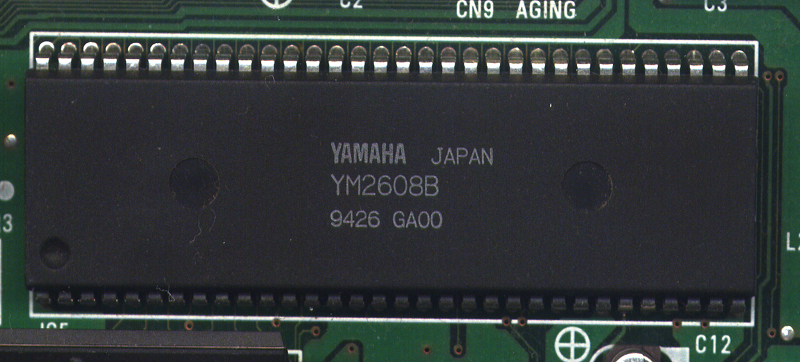
\includegraphics[width=5cm]{img-4.jpg}
    \caption{YAMAHA製音源チップ、YM2608}
  \end{figure}
  FM音源は、周波数変調合成音源と呼ばれる、周波数を変えることで音を出す方式の音源です。\\
  簡単にいうと、ビープ音のような基本の波に手作業で加工を加えて音を作り、その組み合わせで演奏する方式です。\\
  ピーという音しか出せなかったビープ音と比べ、FM音源はさまざまな楽器の音色を再現したり、効果音を作成したりできるために、表現方法に富んでいます。\\
  重厚感と金属感があって、ゲームセンターなどで聞くことができるこれぞゲーム、といった音を出すことができます。\\
  PC-98では、主にYAMAHA社のOPN、OPNAという規格のFM音源が使われていました。\\
  それを搭載した「PC-9801-86」というボードがとても有名で、中後期はこの音源を内蔵した機種が多く発売され、PC-98のFM音源の事実上標準となっていました。\\
  そのような、86ボードおよびそれに準拠した音源の環境のことを「86音源」と言います。\footnote{ここでは便宜上あたかも「PC-9801-86が初めに出て、それに準拠したマシンやボードが出てきた」ような書き方をしていますが、元々、PC-9801-86はPC-9821 A MATEシリーズに内蔵の音源を、音源を搭載していない旧世代の機種で使えるように拡張ボードとして切り出したものです。}\\
  ちなみに、86音源はFM音源だけでなく、後述のPCM音源も搭載しています。\\
  {\bf ・PCM音源 \\}
  PCM音源は、パルス符号変調音源と呼ばれる、音の波形をデジタル化して記録する方式の音源です。\\
  簡単にいうと、現実に鳴っている音をそのまま記録・再生できる方式です。\\
  音の作成をデジタル的に行わなくても良いため、作成難易度が低いほか、表現方法も実質無限大です。\\
  しかし、アナログ的な波の情報をデジタル化するため、現実の音と完全に一致したものを作ることはできません。また、正確な音を記録しようとするほど、必要なデータ量が増えてしまいます。\\
  CDやMDなどの音楽メディアに使われている方式で、現代のPCでも一般的に使われています。\\
  PC-98ではPC-9801-86や後継機種のPC-9801-118にPCM機能が搭載されているほか、後期のWindows環境を想定したPC-9821シリーズの一部にMATE-X PCMというPCM音源が内蔵されました。\\
  {\bf ・\ruby{MIDI}{ミディ}音源 \\}
  MIDI音源は、MIDIという規格を使って音を出す方式の音源です。\\
  元々MIDIとは、楽器同士、または楽器とコンピュータ同士を接続するための規格です。\\
  楽器の持つ音の情報をコンピュータに送り、コンピュータがそれを解釈して音を出すことができます。\\
  ドの音をピアノの音色で鳴らし始めた、鳴らし終わった、レのおとをギターの音色で鳴らし始めた、などの情報が記録されます。\\
  MIDIの音を鳴らすには、MIDIのポートを増設するカードと、MIDI情報を解釈して対応する音を鳴らす音源モジュールが必要です。\\
  MIDIには楽器情報と音階の情報などしか入っておらず、実際の音(=波)の情報は入っていないため、解釈するモジュールによって実際に再生される音が変わります。\\
  高価でしたが、当時はDTM\footnote{デスクトップミュージックの略。コンピュータを使って音楽を作ることを指します。}をする人や、一部の音楽好き、ゲーム好きの間で広がったようです。\\
  PC-98ではRoland社のGSフォーマット、YAMAHA社のXGフォーマットという規格が存在し、2派が互いにしのぎを削っていたようです。\\
  音源モジュールは、Roland社のSoundCanvas(SC)シリーズ、YAMAHA社のMUシリーズなどが有名です。\\
\end{enumerate}
\end{multicols}
\end{document}
